%%%%%%%%%%%%%%%%%%%%%%%%%%%%%%%%%%%%%%%%%
% kaobook
% LaTeX Template
% Version 1.3 (December 9, 2021)
%
% This template originates from:
% https://www.LaTeXTemplates.com
%
% For the latest template development version and to make contributions:
% https://github.com/fmarotta/kaobook
%
% Authors:
% Federico Marotta (federicomarotta@mail.com)
% Based on the doctoral thesis of Ken Arroyo Ohori (https://3d.bk.tudelft.nl/ken/en)
% and on the Tufte-LaTeX class.
% Modified for LaTeX Templates by Vel (vel@latextemplates.com)
%
% License:
% CC0 1.0 Universal (see included MANIFEST.md file)
%
%%%%%%%%%%%%%%%%%%%%%%%%%%%%%%%%%%%%%%%%%

%----------------------------------------------------------------------------------------
%	PACKAGES AND OTHER DOCUMENT CONFIGURATIONS
%----------------------------------------------------------------------------------------

\documentclass[
	a4paper, % Page size
	fontsize=10pt, % Base font size
	twoside=true, % Use different layouts for even and odd pages (in particular, if twoside=true, the margin column will be always on the outside)
	%open=any, % If twoside=true, uncomment this to force new chapters to start on any page, not only on right (odd) pages
	%chapterentrydots=true, % Uncomment to output dots from the chapter name to the page number in the table of contents
	numbers=noenddot, % Comment to output dots after chapter numbers; the most common values for this option are: enddot, noenddot and auto (see the KOMAScript documentation for an in-depth explanation)
]{kaobook}

% Choose the language
\ifxetexorluatex
	\usepackage{polyglossia}
	\setmainlanguage{english}
\else
	\usepackage[english]{babel} % Load characters and hyphenation
\fi
\usepackage[english=british]{csquotes}	% English quotes

% Load packages for testing
\usepackage{blindtext}
% \usepackage{showframe} % Uncomment to show boxes around the text area, margin, header and footer
%\usepackage{showlabels} % Uncomment to output the content of \label commands to the document where they are used

% Load the bibliography package
\usepackage{kaobiblio}
\addbibresource{main.bib} % Bibliography file

% Load mathematical packages for theorems and related environments
\usepackage[framed=true]{kaotheorems}

% Load the package for hyperreferences
\usepackage{kaorefs}

\graphicspath{{examples/documentation/images/}{images/}} % Paths in which to look for images

\makeindex[columns=3, title=Alphabetical Index, intoc] % Make LaTeX produce the files required to compile the index

\makeglossaries % Make LaTeX produce the files required to compile the glossary
\newglossaryentry{computer}{
	name=computer,
	description={is a programmable machine that receives input, stores and manipulates data, and provides output in a useful format}
}

% Glossary entries (used in text with e.g. \acrfull{fpsLabel} or \acrshort{fpsLabel})
\newacronym[longplural={Frames per Second}]{fpsLabel}{FPS}{Frame per Second}
\newacronym[longplural={Tables of Contents}]{tocLabel}{TOC}{Table of Contents}

 % Include the glossary definitions

\makenomenclature % Make LaTeX produce the files required to compile the nomenclature

% Reset sidenote counter at chapters
%\counterwithin*{sidenote}{chapter}

%----------------------------------------------------------------------------------------

\begin{document}

%----------------------------------------------------------------------------------------
%	BOOK INFORMATION
%----------------------------------------------------------------------------------------

\titlehead{General Relativity Notes}

\title[PHYC90012: General Relativity Notes]{PHYC90012: General Relativity Notes}
\subtitle{From lectures given by Prof. Andrew Melatos}

\author[Cameron Taylor]{Cameron Taylor}

\titlehead{\centering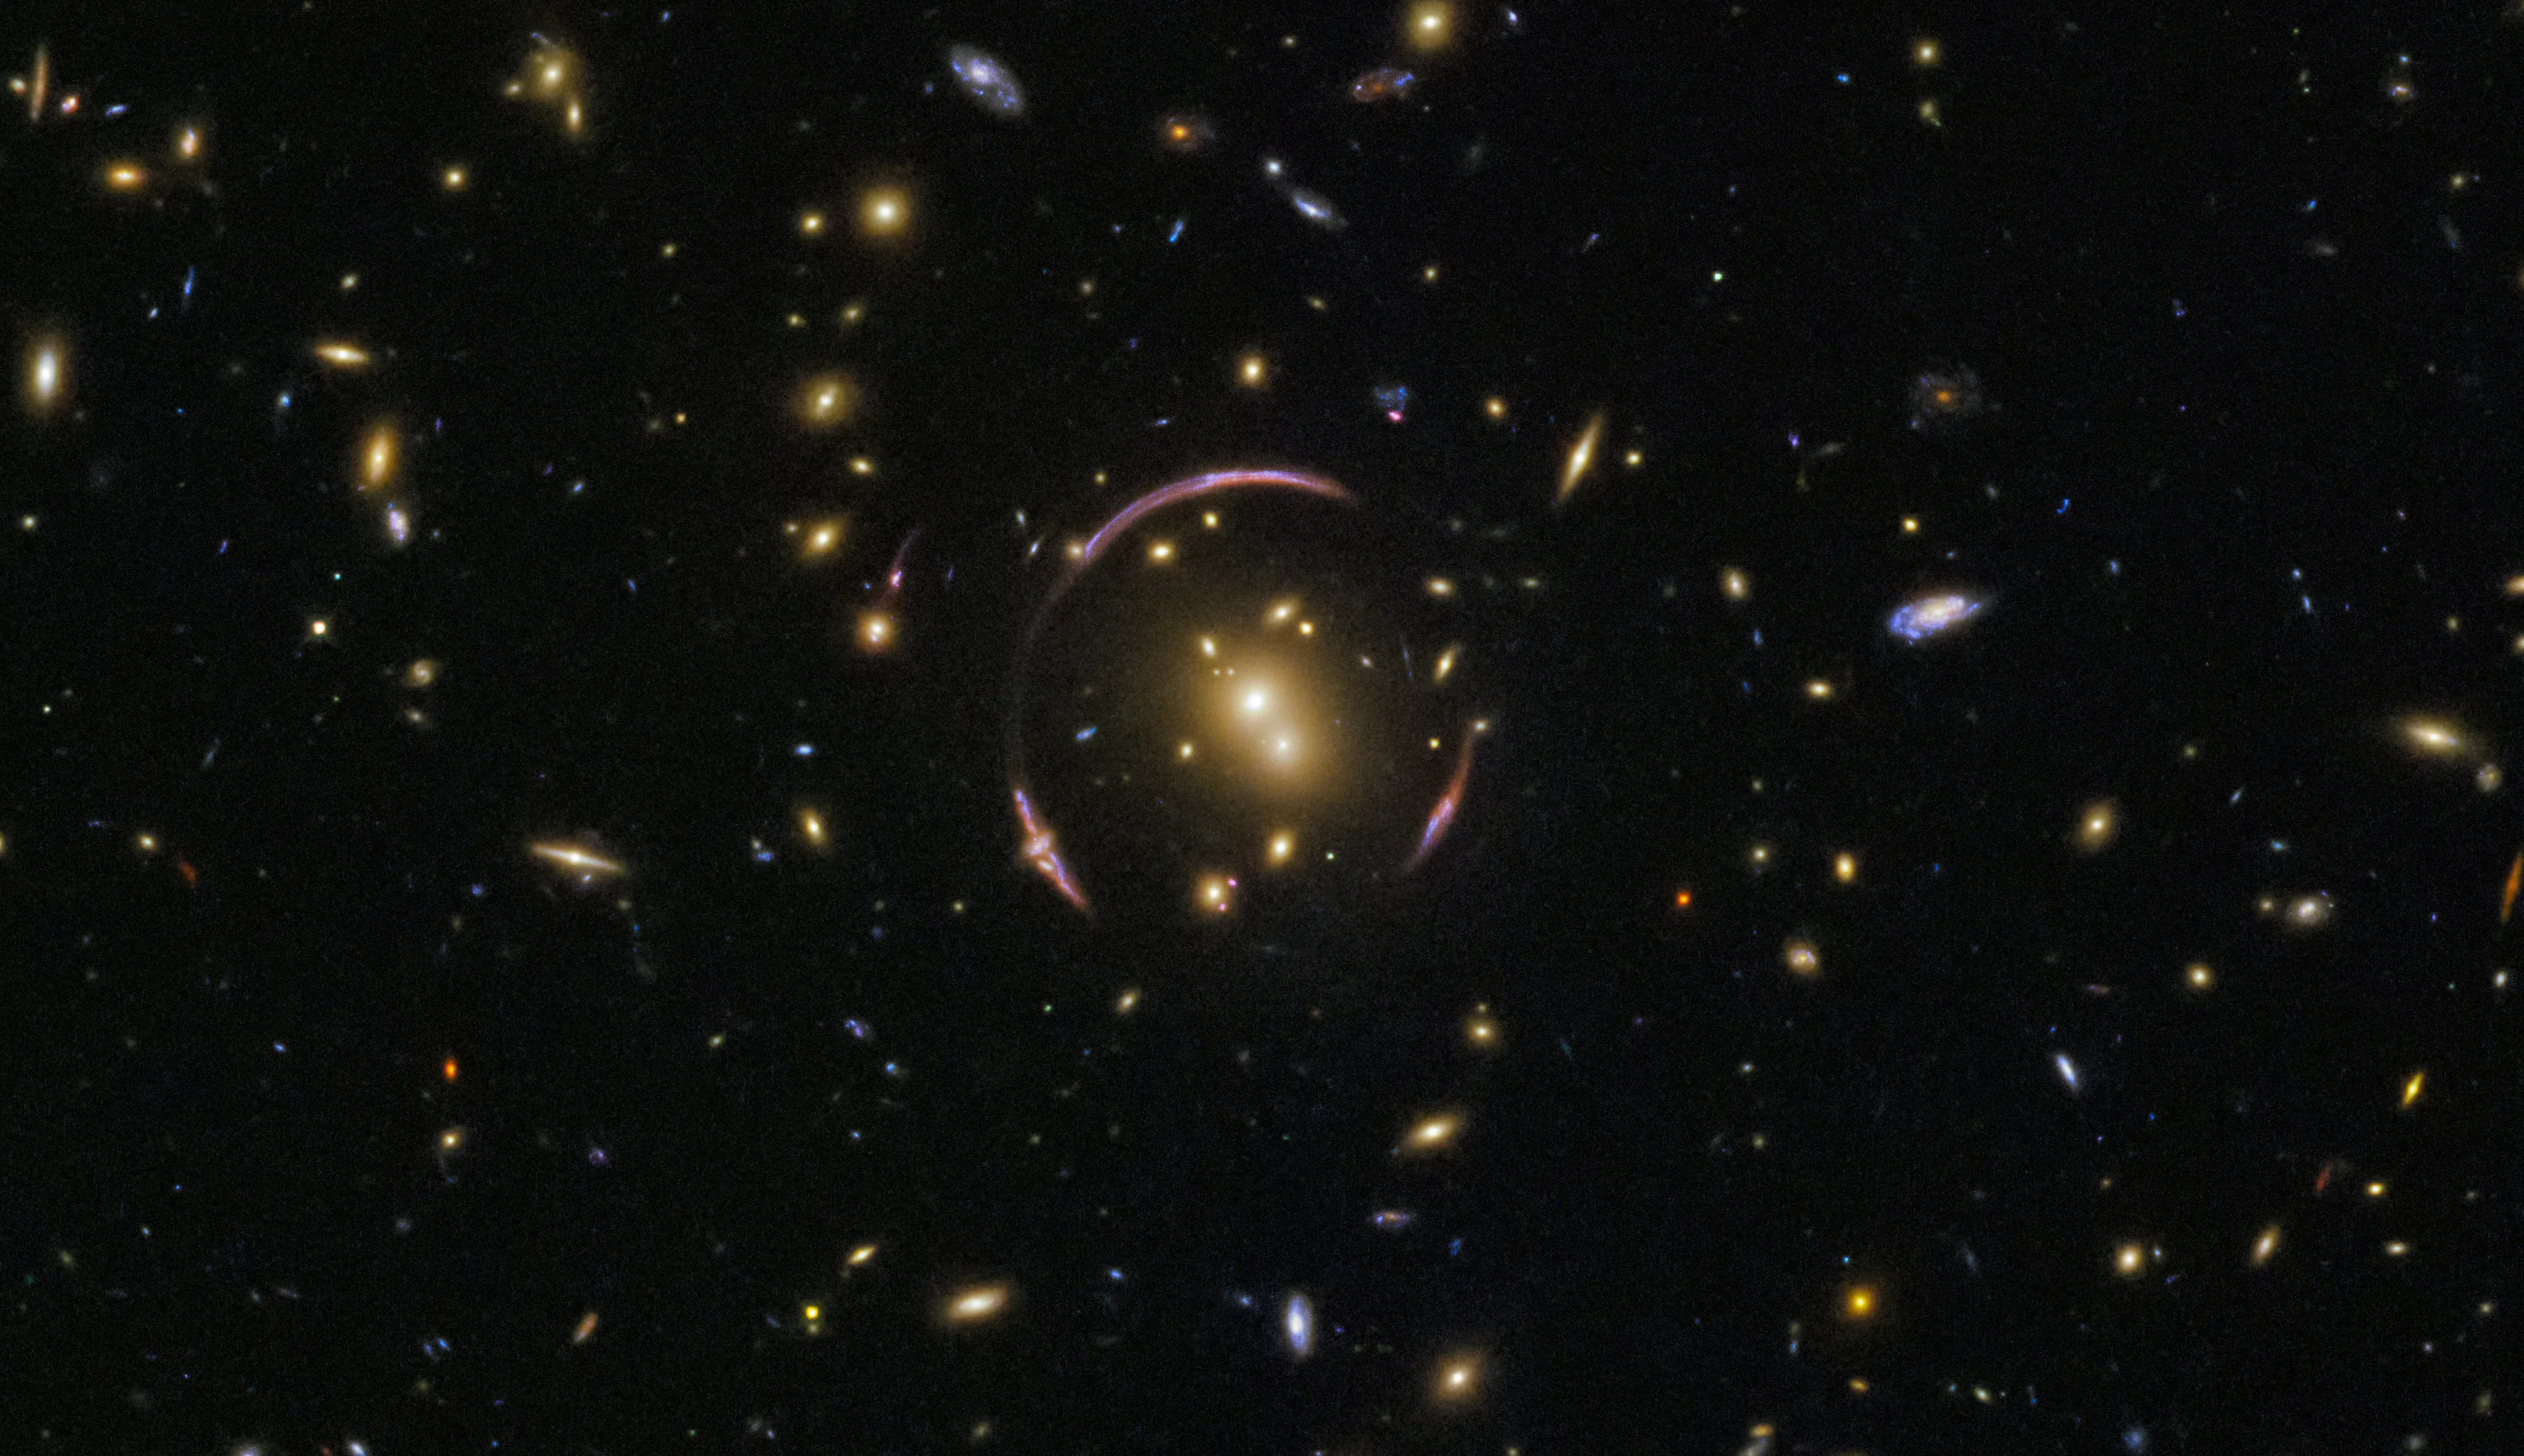
\includegraphics[height=9cm]{images/ring.jpg}}

\date{\today}

% \publishers{An Awesome Publisher}

%----------------------------------------------------------------------------------------

\frontmatter % Denotes the start of the pre-document content, uses roman numerals

%----------------------------------------------------------------------------------------
%	OPENING PAGE
%----------------------------------------------------------------------------------------

%\makeatletter
%\extratitle{
%	% In the title page, the title is vspaced by 9.5\baselineskip
%	\vspace*{9\baselineskip}
%	\vspace*{\parskip}
%	\begin{center}
%		% In the title page, \huge is set after the komafont for title
%		\usekomafont{title}\huge\@title
%	\end{center}
%}
%\makeatother

%----------------------------------------------------------------------------------------
%	COPYRIGHT PAGE
%----------------------------------------------------------------------------------------

% \makeatletter
% \uppertitleback{\@titlehead} % Header

% \lowertitleback{
% 	\textbf{Disclaimer}\\
% 	You can edit this page to suit your needs. For instance, here we have a no copyright statement, a colophon and some other information. This page is based on the corresponding page of Ken Arroyo Ohori's thesis, with minimal changes.
	
% 	\medskip
	
% 	\textbf{No copyright}\\
% 	\cczero\ This book is released into the public domain using the CC0 code. To the extent possible under law, I waive all copyright and related or neighbouring rights to this work.
	
% 	To view a copy of the CC0 code, visit: \\\url{http://creativecommons.org/publicdomain/zero/1.0/}
	
% 	\medskip
	
% 	\textbf{Colophon} \\
% 	This document was typeset with the help of \href{https://sourceforge.net/projects/koma-script/}{\KOMAScript} and \href{https://www.latex-project.org/}{\LaTeX} using the \href{https://github.com/fmarotta/kaobook/}{kaobook} class.
	
% 	The source code of this book is available at:\\\url{https://github.com/fmarotta/kaobook}
	
% 	(You are welcome to contribute!)
	
% 	\medskip
	
% 	\textbf{Publisher} \\
% 	First printed in May 2019 by \@publishers
% }
% \makeatother

%----------------------------------------------------------------------------------------
%	DEDICATION
%----------------------------------------------------------------------------------------

% \dedication{
% 	The harmony of the world is made manifest in Form and Number, and the heart and soul and all the poetry of Natural Philosophy are embodied in the concept of mathematical beauty.\\
% 	\flushright -- D'Arcy Wentworth Thompson
% }

%----------------------------------------------------------------------------------------
%	OUTPUT TITLE PAGE AND PREVIOUS
%----------------------------------------------------------------------------------------

% Note that \maketitle outputs the pages before here

\maketitle

%----------------------------------------------------------------------------------------
%	PREFACE
%----------------------------------------------------------------------------------------

% \chapter*{Preface}
\addcontentsline{toc}{chapter}{Preface} % Add the preface to the table of contents as a chapter

I am of the opinion that every \LaTeX\xspace geek, at least once during 
his life, feels the need to create his or her own class: this is what 
happened to me and here is the result, which, however, should be seen as 
a work still in progress. Actually, this class is not completely 
original, but it is a blend of all the best ideas that I have found in a 
number of guides, tutorials, blogs and tex.stackexchange.com posts. In 
particular, the main ideas come from two sources:

\begin{itemize}
	\item \href{https://3d.bk.tudelft.nl/ken/en/}{Ken Arroyo Ohori}'s 
	\href{https://3d.bk.tudelft.nl/ken/en/nl/ken/en/2016/04/17/a-1.5-column-layout-in-latex.html}{Doctoral 
	Thesis}, which served, with the author's permission, as a backbone 
	for the implementation of this class;
	\item The 
		\href{https://github.com/Tufte-LaTeX/tufte-latex}{Tufte-Latex 
			Class}, which was a model for the style.
\end{itemize}

The first chapter of this book is introductory and covers the most
essential features of the class. Next, there is a bunch of chapters 
devoted to all the commands and environments that you may use in writing 
a book; in particular, it will be explained how to add notes, figures 
and tables, and references. The second part deals with the page layout 
and design, as well as additional features like coloured boxes and 
theorem environments.

I started writing this class as an experiment, and as such it should be 
regarded. Since it has always been intended for my personal use, it may
not be perfect but I find it quite satisfactory for the use I want to 
make of it. I share this work in the hope that someone might find here 
the inspiration for writing his or her own class.

\begin{flushright}
	\textit{Federico Marotta}
\end{flushright}

% \index{preface}

%----------------------------------------------------------------------------------------
%	TABLE OF CONTENTS & LIST OF FIGURES/TABLES
%----------------------------------------------------------------------------------------

\begingroup % Local scope for the following commands

% Define the style for the TOC, LOF, and LOT
%\setstretch{1} % Uncomment to modify line spacing in the ToC
%\hypersetup{linkcolor=blue} % Uncomment to set the colour of links in the ToC
\setlength{\textheight}{230\hscale} % Manually adjust the height of the ToC pages

% Turn on compatibility mode for the etoc package
\etocstandarddisplaystyle % "toc display" as if etoc was not loaded
\etocstandardlines % "toc lines" as if etoc was not loaded

\tableofcontents % Output the table of contents

\listoffigures % Output the list of figures


% Comment both of the following lines to have the LOF and the LOT on different pages
\let\cleardoublepage\bigskip
\let\clearpage\bigskip

\listoftables % Output the list of tables

\endgroup

%----------------------------------------------------------------------------------------
%	MAIN BODY
%----------------------------------------------------------------------------------------

\mainmatter % Denotes the start of the main document content, resets page numbering and uses arabic numbers
\setchapterstyle{kao} % Choose the default chapter heading style

% \setchapterpreamble[u]{\margintoc}
\chapter{Introduction}
\labch{intro}

\section{The Main Ideas}

Many modern printed textbooks have adopted a layout with prominent 
margins where small figures, tables, remarks and just about everything 
else can be displayed. Arguably, this layout helps to organise the 
	discussion by separating the main text from the ancillary material, 
	which at the same time is very close to the point in the text where 
	it is referenced.

This document does not aim to be an apology of wide margins, for there 
are many better suited authors for this task; the purpose of all these 
words is just to fill the space so that the reader can see how a book 
written with the kaobook class looks like. Meanwhile, I shall also try 
to illustrate the features of the class.

The main ideas behind kaobook come from this 
\href{https://3d.bk.tudelft.nl/ken/en/2016/04/17/a-1.5-column-layout-in-latex.html}{blog 
	post}, and actually the name of the class is dedicated to the author 
of the post, Ken Arroyo Ohori, which has kindly allowed me to create a 
class based on his thesis. Therefore, if you want to know more reasons 
to prefer a 1.5-column layout for your books, be sure to read his blog 
post.

Another source of inspiration, as you may have noticed, is the 
\href{https://github.com/Tufte-LaTeX/tufte-latex}{Tufte-Latex Class}. 
The fact that the design is similar is due to the fact that it is very 
difficult to improve something which is already so good. However, I like 
to think that this class is more flexible than Tufte-Latex. For 
instance, I have tried to use only standard packages and to implement as 
little as possible from scratch;\sidenote{This also means that 
understanding and contributing to the class development is made easier. 
Indeed, many things still need to be improved, so if you are interested, 
check out the repository on github!} therefore, it should be pretty easy 
to customise anything, provided that you read the documentation of the 
package that provides that feature.

In this book I shall illustrate the main features of the class and 
provide information about how to use and change things. Let us get 
started.

\section{What This Class Does}
\labsec{does}

The \Class{kaobook} class focuses more about the document structure than 
about the style. Indeed, it is a well-known \LaTeX\xspace principle that 
structure and style should be separated as much as possible (see also 
\vrefsec{doesnot}). This means that this class will only provide 
commands, environments and in general, the opportunity to do things, 
which the user may or may not use. Actually, some stylistic matters are 
embedded in the class, but the user is able to customise them with ease.

The main features are the following:

\begin{description}
	\item[Page Layout] The text width is reduced to improve readability 
	and make space for the margins, where any sort of elements can be 
	displayed.
	\item[Chapter Headings] As opposed to Tufte-Latex, we provide a 
	variety of chapter headings among which to choose; examples will be 
	seen in later chapters.
	\item[Page Headers] They span the whole page, margins included, and, 
	in twoside mode, display alternatively the chapter and the section 
	name.\sidenote[][-2mm]{This is another departure from Tufte's 
	design.}
	\item[Matters] The commands \Command{frontmatter}, 
	\Command{mainmatter} and \Command{backmatter} have been redefined in 
	order to have automatically wide margins in the main matter, and 
	narrow margins in the front and back matters. However, the page 
	style can be changed at any moment, even in the middle of the 
	document.
	\item[Margin text] We provide commands \Command{sidenote} and 
	\Command{marginnote} to put text in the 
	margins.\sidenote[][-2mm]{Sidenotes (like this!) are numbered while 
	marginnotes are not}
	\item[Margin figs/tabs] A couple of useful environments is 
	\Environment{marginfigure} and \Environment{margintable}, which, not 
	surprisingly, allow you to put figures and tables in the margins 
	(\cfr \reffig{marginmonalisa}).
	\item[Margin toc] Finally, since we have wide margins, why don't add 
	a little table of contents in them? See \Command{margintoc} for 
	that.
	\item[Hyperref] \Package{hyperref} is loaded and by default we try 
	to add bookmarks in a sensible way; in particular, the bookmarks 
	levels are automatically reset at \Command{appendix} and 
	\Command{backmatter}. Moreover, we also provide a small package to 
	ease the hyperreferencing of other parts of the text.
	\item[Bibliography] We want the reader to be able to know what has 
	been cited without having to go to the end of the document every 
	time, so citations go in the margins as well as at the end, as in 
	Tufte-Latex. Unlike that class, however, you are free to customise 
	the citations as you wish.
\end{description}

\begin{marginfigure}[-5.5cm]
	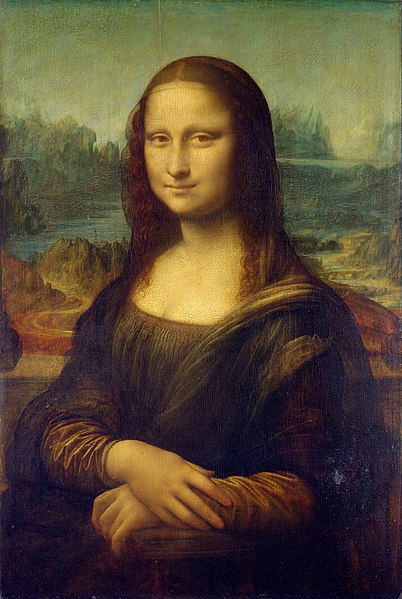
\includegraphics{monalisa}
	\caption[The Mona Lisa]{The Mona Lisa.\\ 
	\url{https://commons.wikimedia.org/wiki/File:Mona_Lisa,_by_Leonardo_da_Vinci,_from_C2RMF_retouched.jpg}}
	\labfig{marginmonalisa}
\end{marginfigure}

The order of the title pages, table of contents and preface can be 
easily changed, as in any \LaTeX\ document. In addition, the class is 
based on \KOMAScript's \Class{scrbook}, therefore it inherits all the 
goodies of that.

\section{What This Class Does Not Do}
\labsec{doesnot}

As anticipated, further customisation of the book is left to the user. 
Indeed, every book may have sidenotes, margin figures and so on, but 
each book will have its own fonts, toc style, special environments and 
so on. For this reason, in addition to the class, we provide only 
sensible defaults, but if these features are not needed, they can be 
left out. These special packages are located in the \Path{style} 
directory, which is organised as follows:

\begin{description}
	\item[kao.sty] This package contains the most important definitions 
	of macros and specifications of page layout. It is the heart of the 
	\Class{kaobook}.
	\item[kaobiblio.sty] Contains commands to add citations and 
	customise the bibliography.
	\item[packages.sty] Loads additional packages to decorate the 
	writing with special contents (for instance, the \Package{listing} 
	package is loaded here as it is not required in every book). There 
	are also defined some useful commands to print the same words always 
	in the same way, \eg latin words in italics or \Package{packages} in 
	verbatim.
	\item[kaorefs.sty] Some useful commands to manage labeling and 
	referencing, again to ensure that the same elements are referenced 
	always in a consistent way.
	\item[environments.sty] Provides special environments, like boxes. 
	Both simple and complex environments are available; by complex we 
	mean that they are endowed with a counter, floating and can be put 
	in a special table of contents.\sidenote[][-2mm]{See 
	\vrefch{mathematics} for some examples.}
	\item[theorems.sty] The style of mathematical environments. 
	Actually, there are two such packages: one is for plain theorems,
	\ie the theorems are printed in plain text; the other uses 
	\Package{mdframed} to draw a box around theorems. You can plug the 
	most appropriate style into its document.
\end{description}

\marginnote[2mm]{The audacious users might feel tempted to edit some of 
these packages. I'd be immensely happy if they sent me examples of what 
they have been able to do!}

In the rest of the book, I shall assume that the reader is not a novice 
in the use of \LaTeX, and refer to the documentation of the packages 
used in this class for things that are already explained there. 
Moreover, I assume that the reader is willing to make minor edits to the 
provided packages for styles, environments and commands, if he or she 
does not like the default settings.

\section{How to Use This Class}

Either if you are using the template from 
\href{http://latextemplates.org/template/kaobook}{latextemplates}, or if 
you cloned the GitHub 
\href{https://www.github.com/fmarotta/kaobook}{repository}, there are 
infinite ways to use the \Class{kaobook} class in practice, but we will 
discuss only two of them. The first is to find the \Path{main.tex} file 
which I used to write this book, and edit it; this will probably involve 
a lot of text-deleting, copying-and-pasting, and rewriting. The second 
way is to start almost from scratch and use the \Path{skeleton.tex} 
file, which is a cleaned-up version of the \Path{main.tex}; even if you 
choose the second way, you may find it useful to draw inspiration from 
the \Path{main.tex} file.

To compile the document, assuming that its name is \Path{main.tex}, you 
will have to run the following sequence of commands:

\begin{lstlisting}[style=kaolstplain,linewidth=1.5\textwidth]
pdflatex main # Compile template
makeindex main.nlo -s nomencl.ist -o main.nls # Compile nomenclature
makeindex main # Compile index
biber main # Compile bibliography
makeglossaries main # Compile glossary
pdflatex main # Compile template again
pdflatex main # Compile template again
\end{lstlisting}

You may need to compile the template some more times in order for some 
errors to disappear. For any support requests, please ask a question on 
\url{tex.stackexchange.org} with the tag \enquote{kaobook}, open an 
issue on GitHub, or contact the author via e-mail.


% \pagelayout{wide} % No margins
% \addpart{Class Options, Commands and Environments}
% \pagelayout{margin} % Restore margins

% \setchapterpreamble[u]{\margintoc}
\chapter{Class Options}
\labch{options}

In this chapter I will describe the most common options used, both the 
ones inherited from \Class{scrbook} and the \Class{kao}-specific ones. 
Options passed to the class modifies its default behaviour; beware 
though that some options may lead to unexpected results\ldots

\section{\Class{KOMA} Options}

The \Class{kaobook} class is based on \Class{scrbook}, therefore it 
understands all of the options you would normally pass to that class. If 
you have a lot of patience, you can read the \KOMAScript\xspace 
guide.\sidenote{The guide can be downloaded from 
\url{https://ctan.org/pkg/koma-script?lang=en}.} Actually, the reading 
of such guide is suggested as it is very instructive.

Every \KOMAScript\xspace option you pass to the class when you load it 
is automatically activated. In addition, in \Class{kaobook} some options 
have modified default values. For instance, the font size is 9.5pt and 
the paragraphs are separated by space,\sidenote[][-7mm]{To be precise, 
they are separated by half a line worth of space: the \Option{parskip} 
value is \enquote{half}.} not marked by indentation.

\section{\Class{kao} Options}

In the future I plan to add more options to set the paragraph formatting 
(justified or ragged) and the position of the margins (inner or outer in 
twoside mode, left or right in oneside mode).\sidenote{As of now, 
paragraphs are justified, formatted with \Command{singlespacing} (from 
the \Package{setspace} package) and \Command{frenchspacing}.}

I take this opportunity to renew the call for help: everyone is 
encouraged to add features or reimplement existing ones, and to send me 
the results. You can find the GitHub repository at 
\url{https://github.com/fmarotta/kaobook}.

\begin{kaobox}[frametitle=To Do]
Implement the \Option{justified} and \Option{margin} options. To be 
consistent with the \KOMAScript\xspace style, they should accept a 
simple switch as a parameter, where the simple switch should be 
\Option{true} or \Option{false}, or one of the other standard values for 
simple switches supported by \KOMAScript. See the \KOMAScript\xspace 
documentation for further information.
\end{kaobox}

The above box is an example of a \Environment{kaobox}, which will be 
discussed more thoroughly in \frefch{mathematics}. Throughout the book I 
shall use these boxes to remarks what still needs to be done.

\section{Other Things Worth Knowing}

A bunch of packages are already loaded in the class because they are 
needed for the implementation. These include:

\begin{itemize}
	\item etoolbox
	\item calc
	\item xifthen
	\item xkeyval
	\item xparse
	\item xstring
\end{itemize}

Many more packages are loaded, but they will be discussed in due time. 
Here, we will mention only one more set of packages, needed to change 
the paragraph formatting (recall that in the future there will be 
options to change this). In particular, the packages we load are:

\begin{itemize}
	\item ragged2e
	\item setspace
	\item hyphenat
	\item microtype
	\item needspace
	\item xspace
	\item xcolor (with options \Option{usenames,dvipsnames})
\end{itemize}

Some of the above packages do not concern paragraph formatting, but we 
nevertheless grouped them with the others. By default, the main text is 
justified and formatted with singlespacing and frenchspacing; the margin 
text is the same, except that the font is a bit smaller.

As a last warning, please be aware that the \Package{cleveref} package 
is not compatible with \Class{kaobook}. You should use the commands 
discussed in \refsec{hyprefs} instead.

\section{Document Structure}

We provide optional arguments to the \Command{title} and 
\Command{author} commands so that you can insert short, plain text 
versions of this fields, which can be used, typically in the half-title 
or somewhere else in the front matter, through the commands 
\Command{@plaintitle} and \Command{@plainauthor}, respectively. The PDF 
properties \Option{pdftitle} and \Option{pdfauthor} are automatically 
set by hyperref to the plain values if present, otherwise to the normal 
values.\sidenote[][*-1]{We think that this is an important point so 
we remark it here. If you compile the document with pdflatex, the PDF 
metadata will be altered so that they match the plain title and author 
you have specified; if you did not specify them, the metadata will be 
set to the normal title and author.}

There are defined two page layouts, \Option{margin} and \Option{wide}, 
and two page styles, \Option{plain} and \Option{fancy}. The layout 
basically concern the width of the margins, while the style refers to 
headers and footer; these issues will be 
discussed in \frefch{layout}.\sidenote[][6mm]{For now, suffice it to say that pages with 
the \Option{margin} layout have wide margins, while with the 
\Option{wide} layout the margins are absent. In \Option{plain} pages the 
headers and footer are suppressed, while in \Option{fancy} pages there 
is a header.} 

The commands \Command{frontmatter}, \Command{mainmatter}, and 
\Command{backmatter} have been redefined in order to automatically 
change page layout and style for these sections of the book. The front 
matter uses the \Option{margin} layout and the \Option{plain} page 
style. In the mainmatter the margins are wide and the headings are 
fancy. In the appendix the style and the layout do not change; however 
we use \Command{bookmarksetup\{startatroot\}} so that the bookmarks of 
the chapters are on the root level (without this, they would be under 
the preceding part). In the backmatter the margins shrink again and we 
also reset the bookmarks root.

% \setchapterpreamble[u]{\margintoc}
\chapter{Margin Stuff}

Sidenotes are a distinctive feature of all 1.5-column-layout books. 
Indeed, having wide margins means that some material can be displayed 
there. We use margins for all kind of stuff: sidenotes, marginnotes, 
small tables of contents, citations, and, why not?, special boxes and 
environments.

\section{Sidenotes}

Sidenotes are like footnotes, except that they go in the margin, where 
they are more readable. To insert a sidenote, just use the command 
\Command{sidenote\{Text of the note\}}. You can specify a 
mark\sidenote[O]{This sidenote has a special mark, a big O!} with \\ 
\Command{sidenote[mark]\{Text\}}, but you can also specify an offset, 
which moves the sidenote upwards or downwards, so that the full syntax is:

\begin{lstlisting}[style=kaolstplain]
\sidenote[mark][offset]{Text}
\end{lstlisting}

If you use an offset, you always have to add the brackets for the mark, 
but they can be empty.\sidenote{If you want to know more about the usage 
of the \Command{sidenote} command, read the documentation of the 
\Package{sidenotes} package.}

In \Class{kaobook} we copied a feature from the \Package{snotez} 
package: the possibility to specify a multiple of \Command{baselineskip} 
as an offset. For example, if you want to enter a sidenote with the 
normal mark and move it upwards one line, type:

\begin{lstlisting}[style=kaolstplain]
\sidenote[][*-1]{Text of the sidenote.}
\end{lstlisting}

As we said, sidenotes are handled through the \Package{sidenotes} 
package, which in turn relies on the \Package{marginnote} package.

\section{Marginnotes}

This command is very similar to the previous one. You can create a 
marginnote with \Command{marginnote[offset]\{Text\}}, where the offset 
argument can be left out, or it can be a multiple of 
\Command{baselineskip},\marginnote[-1cm]{While the command for margin 
notes comes from the \Package{marginnote} package, it has been redefined 
in order to change the position of the optional offset argument, which 
now precedes the text of the note, whereas in the original version it 
was at the end. We have also added the possibility to use a multiple of 
\Command{baselineskip} as offset. These things were made only to make 
everything more consistent, so that you have to remember less things!} 
\eg

\begin{lstlisting}[style=kaolstplain]
\marginnote[-12pt]{Text} or \marginnote[*-3]{Text}
\end{lstlisting}

\begin{kaobox}[frametitle=To Do]
A small thing that needs to be done is to renew the \Command{sidenote} 
command so that it takes only one optional argument, the offset. The 
special mark argument can go somewhere else. In other words, we want the 
syntax of \Command{sidenote} to resemble that of \Command{marginnote}.
\end{kaobox}

We load the packages \Package{marginnote}, \Package{marginfix} and 
\Package{placeins}. Since \Package{sidenotes} uses \Package{marginnote}, 
what we said for marginnotes is also valid for sidenotes. Side- and 
margin- notes are shifted slightly upwards 
(\Command{renewcommand\{\textbackslash marginnotevadjust\}\{3pt\}}) in 
order to align them to the bottom of the line of text where the note is 
issued. Importantly, both sidenotes and marginnotes are defined as 
floating if the optional argument (\ie the vertical offset) is left 
blank, but if the offset is specified they are not floating. Recall that 
floats cannot be nested, so in some rare cases you may encounter errors 
about lost floats; in those cases, remember that sidenotes and 
marginnotes are floats. To solve the problem, it may be possible to 
transform them into non-floating elements by specifying an offset of 
0pt.

\section{Footnotes}

Even though they are not displayed in the margin, we will discuss about 
footnotes here, since sidenotes are mainly intended to be a replacement 
of them. Footnotes force the reader to constantly move from one area of 
the page to the other. Arguably, marginnotes solve this issue, so you 
should not use footnotes. Nevertheless, for completeness, we have left 
the standard command \Command{footnote}, just in case you want to put a 
footnote once in a while.\footnote{And this is how they look like. 
Notice that in the PDF file there is a back reference to the text; 
pretty cool, uh?}

\section{Margintoc}

Since we are talking about margins, we introduce here the 
\Command{margintoc} command, which allows one to put small table of 
contents in the margin. Like other commands we have discussed, 
\Command{margintoc} accepts a parameter for the vertical offset, like 
so: \Command{margintoc[offset]}.

The command can be used in any point of the document, but we think it 
makes sense to use it just at the beginning of chapters or parts. In 
this document I make use of a \KOMAScript\xspace feature and put it in 
the chapter preamble, with the following code:

\marginnote{The font used in the margintoc is the same as the one for 
	the chapter entries in the main table of contents at the beginning 
	of the document.}

\begin{lstlisting}[style=kaolstplain]
\setchapterpreamble[u]{\margintoc}
\chapter{Chapter title}
\end{lstlisting}

As the space in the margin is a valuable resource, there is the 
possibility to print a shorter version of the title in the margin toc. 
Thus, there are in total three possible versions for the title of a 
section (or subsection): the one for the main text, the one for the main 
table of contents, and the one for the margintoc. These versions can be 
specified at the same time when the section is created in the source 
\TeX file:
\begin{lstlisting}[style=kaolstplain]
\section[alternative-title-for-toc]{title-as-written-in-text}[alternative-title-for-margintoc]
\end{lstlisting}

By default, the margintoc includes sections and subsections.
If you only want to show sections, add
\begin{lstlisting}[style=kaolstplain]
\setcounter{margintocdepth}{\sectiontocdepth}
\end{lstlisting}
somewhere in your preamble.

\section{Marginlisting}

On some occasions it may happen that you have a very short piece of code 
that doesn't look good in the body of the text because it breaks the 
flow of narration: for that occasions, you can use a 
\Environment{marginlisting}. The support for this feature is still 
limited, especially for the captions, but you can try the following 
code:

\begin{marginlisting}[-1.35cm]
	\caption{An example of a margin listing.}
	\vspace{0.6cm}
	\begin{lstlisting}[language=Python,style=kaolstplain]
print("Hello World!")
	\end{lstlisting}
\end{marginlisting}

\begin{verbatim}
\begin{marginlisting}[-0.5cm]
	\caption{My caption}
	\vspace{0.2cm}
	\begin{lstlisting}[language=Python,style=kaolstplain]
	... code ...
	\end{lstlisting}
\end{marginlisting}
\end{verbatim}

Unfortunately, the space between the caption and the listing must be 
adjusted manually; if you find a better way, please let me know.

Not only textual stuff can be displayed in the margin, but also figures. 
Those will be the focus of the next chapter.

% \setchapterimage[7.5cm]{seaside}
\setchapterpreamble[u]{\margintoc}
%\chapter[Figures and Tables]{Figures and Tables\footnotemark[0]}
\chapter{Figures and Tables}

\footnotetext{The credits for the image above the chapter title go to:
	Bushra Feroz, CC~BY-SA~4.0, \url{https://commons.wikimedia.org/w/index.php?curid=68724647}}

\section{Normal Figures and Tables}

Figures and tables can be inserted just like in any standard 
\LaTeX\xspace document. The \Package{graphicx} package is already loaded 
and configured in such a way that the figure width is equal to the 
textwidth and the height is adjusted in order to maintain the original 
aspect ratio. As you may have imagined, the captions will be 
positioned\ldots well, in the margins. This is achieved with the help of 
the \Package{floatrow} package.

Here is a picture of Mona Lisa (\reffig{normalmonalisa}), as an example. 
The captions are formatted as the margin- and the side-notes; If you 
want to change something about captions you can use the command 
\Command{captsetup} from the \Package{caption} package. Remember that if 
you want to reference a figure, the label must come \emph{after} the 
caption!

\begin{figure}[hb]
	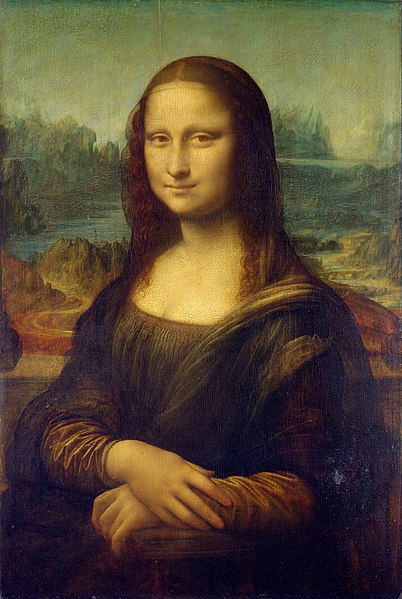
\includegraphics[width=0.45\textwidth]{monalisa}
	\caption[Mona Lisa, again]{It's Mona Lisa again. \blindtext}
	\labfig{normalmonalisa}
\end{figure}

While the format of the caption is managed by \Package{caption}, its 
position is handled by the \Package{floatrow} package. Achieving this 
result has been quite hard, but now I am pretty satisfied. In two-side 
mode, the captions are printed in the correct margin.

Tables can be inserted just as easily as figures, as exemplified by the 
following code:

\begin{lstlisting}[caption={Caption of a listing.}]
\begin{table}
\begin{tabular}{ c c c c }
	\toprule
	col1 & col2 & col3 & col 4 \\
	\midrule
	\multirow{3}{4em}{Multiple row} & cell2 & cell3 & cell4\\ &
	cell5 & cell6 & cell7 \\ &
	cell8 & cell9 & cell10 \\
	\multirow{3}{4em}{Multiple row} & cell2 & cell3 & cell4 \\ &
	cell5 & cell6 & cell7 \\ &
	cell8 & cell9 & cell10 \\
	\bottomrule
\end{tabular}
\end{table}
\end{lstlisting}

which results in the useless \vreftab{useless}.

\begin{table}[ht]
\caption[A useless table]{A useless table.}
\labtab{useless}
\begin{tabular}{ c c c c }
	\toprule
	col1 & col2 & col3 & col 4 \\
	\midrule
	\multirow{3}{4em}{Multiple row} & cell2 & cell3 & cell4\\ &
	cell5 & cell6 & cell7 \\ &
	cell8 & cell9 & cell10 \\
	\multirow{3}{4em}{Multiple row} & cell2 & cell3 & cell4 \\ &
	cell5 & cell6 & cell7 \\ &
	cell8 & cell9 & cell10 \\
	\bottomrule
\end{tabular}
\end{table}

I don't have much else to say, so I will just insert some blind text. 
\blindtext

\section{Margin Figures and Tables}

Marginfigures can be inserted with the environment 
\Environment{marginfigure}. In this case, the whole picture is confined 
to the margin and the caption is below it. \reffig{marginmonalisa} is 
obtained with something like this:

\begin{lstlisting}[caption={Another caption.}]
\begin{marginfigure}
	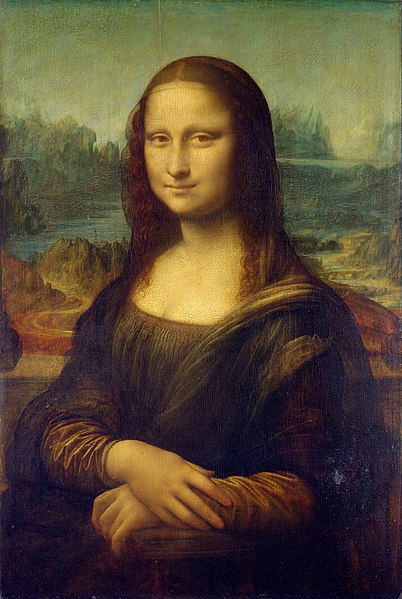
\includegraphics{monalisa}
	\caption[The Mona Lisa]{The Mona Lisa.}
	\labfig{marginmonalisa}
\end{marginfigure}
\end{lstlisting}

There is also the \Environment{margintable} environment, of which 
\reftab{anotheruseless} is an example. Notice how you can place the 
caption above the table by just placing the \Command{caption} command 
before beginning the \Environment{tabular} environment. Usually, figure 
captions are below, while table captions are above. This rule is also 
respected for normal figures and tables: the captions are always on the 
side, but for figure they are aligned to the bottom, while for tables to 
the top.

\begin{margintable}
\caption[Another useless table]{Another useless table.}
\labtab{anotheruseless}
\raggedright
\begin{tabular}{ c c c c }
	\hline
	col1 & col2 & col3 \\
	\hline
	\multirow{3}{4em}{Multiple row} & cell2 & cell3 \\ & cell5 & cell6 
	\\ & cell8 & cell9 \\ \hline
\end{tabular}
\end{margintable}

Marginfigures and tables can be positioned with an optional offset 
command, like so:

\begin{lstlisting}
\begin{marginfigure}[offset]
	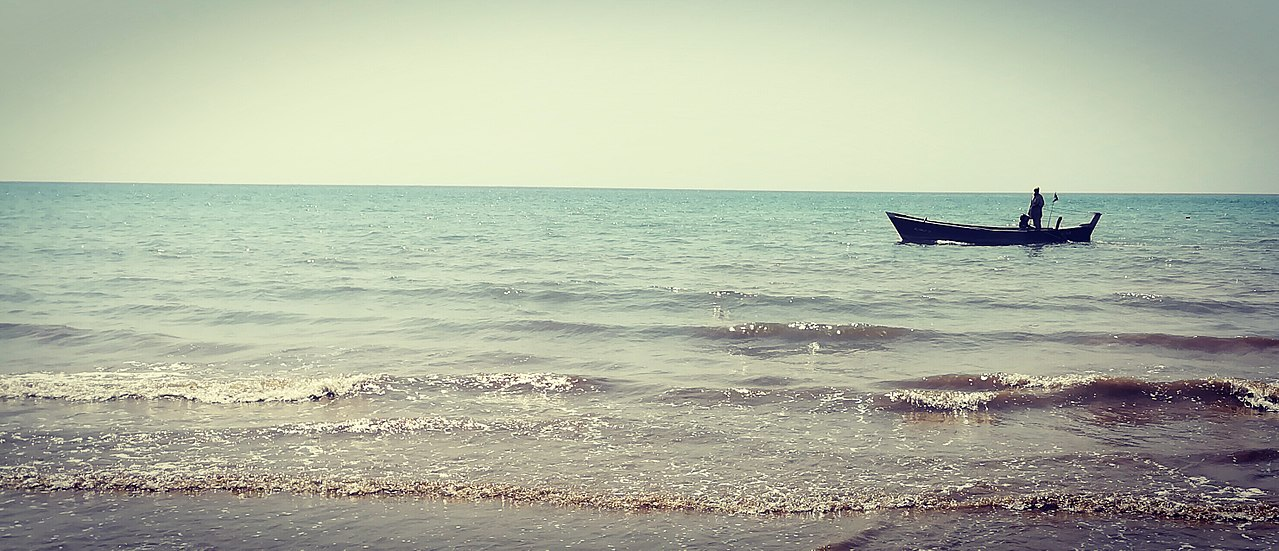
\includegraphics{seaside}
\end{marginfigure}
\end{lstlisting}

Offset ca be either a measure or a multiple of \Command{baselineskip}, 
much like with \Command{sidenote}, \Command{marginnote} and 
\Command{margintoc}.\todo{Improve this part.} If you are wondering how I 
inserted this orange bubble, have a look at the \Package{todo} package.

\section{Wide Figures and Tables}

With the environments \Environment{figure*} and \Environment{table*} you 
can insert figures which span the whole page width. For example, here 
are a wide figure and a wide table.

\begin{figure*}[h!]
	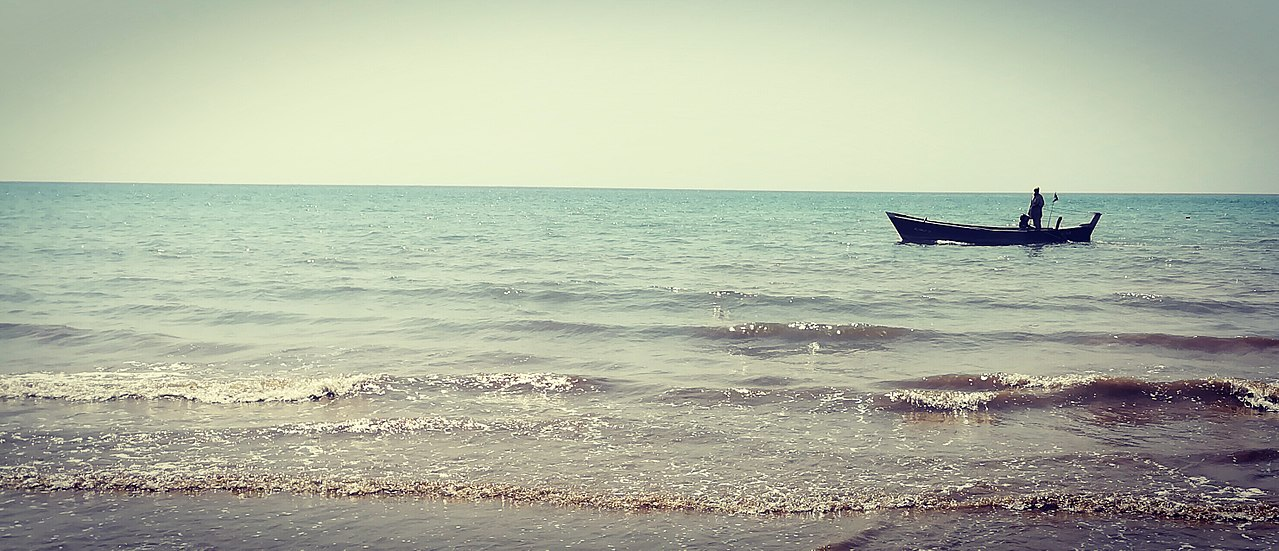
\includegraphics{seaside}
	\caption[A wide seaside]{A wide seaside, and a wide caption.
		Credits: By Bushra Feroz, CC BY-SA 4.0, \url{https://commons.wikimedia.org/w/index.php?curid=68724647}}
\end{figure*}

\begin{table*}[h!]
    \caption{A wide table with invented data about three people living in the UK. Note that wide figures and tables are centered and their caption also extends into the margin.}
    \begin{tabular}{p{2.0cm} p{2.0cm} p{2.0cm} p{2.0cm} p{2.0cm} p{2.0cm} p{1.5cm}}
        \toprule
        Name    & Surname   & Job       & Salary           & Age   & Height    & Country \\
        \midrule
        Alice   & Red       & Writer    & 4.000 \pounds    & 34    & 167 cm     & England \\
        Bob     & White     & Bartender & 2.000 \pounds    & 24    & 180 cm     & Scotland \\
        Drake   & Green     & Scientist & 4.000 \pounds    & 26    & 175 cm     & Wales \\
        \bottomrule
    \end{tabular}
\end{table*}

It is the user's responsibility to adjust the width of the table, if 
necessary, until it is aesthetically pleasing. The previous table was 
obtained with the following code:

\begin{lstlisting}[caption=How to typeset a wide table]
\begin{table*}[h!]
    \caption{A wide table with invented data about three people living in the UK. Note that wide figures and tables are centered and their caption also extends into the margin.}
    \begin{tabular}{p{2.0cm} p{2.0cm} p{2.0cm} p{2.0cm} p{2.0cm} p{2.0cm} p{1.5cm}}
        \toprule
        Name    & Surname   & Job       & Salary           & Age   & Height    & Country \\
        \midrule
        Alice   & Red       & Writer    & 4.000 \pounds    & 34    & 167 cm     & England \\
        Bob     & White     & Bartender & 2.000 \pounds    & 24    & 180 cm     & Scotland \\
        Drake   & Green     & Scientist & 4.000 \pounds    & 26    & 175 cm     & Wales \\
        \bottomrule
    \end{tabular}
\end{table*}
\end{lstlisting}

The \Package{floatrow} package provides the \enquote{H} specifier to 
instruct \LaTeX to position the figure (or table) in precisely the same 
position it occupies in the source code. However, this specifier does 
not work with wide figures or tables: you should use \enquote{h!} 
instead, like so: \lstinline|\begin{figure*}[h!]|.

You may have noticed the full width image at the very beginning of this
chapter: that, however, is set up in an entirely different way, which
you'll read about in \vrefch{layout}.

\Class{kaobook} also supports paginated tables (have a look at the 
\Package{longtable} package). The 
\Environment{longtable}\sidenote{Interestingly, \Environment{longtable}s 
may require up to four rounds of compilation before they are typeset 
correctly.} environment behaves a bit differently from 
\Environment{table}, in that \Environment{longtable} encompasses both 
\Environment{table} and \Environment{tabular}, so that you can write, 
\eg,

\begin{lstlisting}[caption=Example of a longtable]
\begin{longtable}{|l c c|}
    \hline
    One & Two & Three \\
    Left & Center & Center \\
    \hline
    \caption{Caption of the longtable.}
\end{longtable}
\end{lstlisting}

to obtain the following table:
\begin{longtable}{|l c c|}
    \hline
    One & Two & Three \\
    Left & Center & Center \\
    \hline
    \caption{Caption of the longtable.}
\end{longtable}

The caption of a \Environment{longtable} is always positioned below the 
table, and it has the same width as the text (it doesn't extend into the 
margin). However, sometimes you may need a \Environment{longtable} that 
is so wide that it trespass into the margins; in those cases, you may 
want to also increase the width of the caption. To do so, you'll have to 
write two additional commands, one before and one after the 
\Environment{longtable}:

\begin{lstlisting}[caption=Increasing the width of the caption of a \Environment{longtable}.]
\floatsetup[longtable]{margins=centering,LTcapwidth=table} % Add this line before the longtable to increase the caption width
\begin{longtable}{lp{8cm}p{5cm}p{2cm}}
...
\end{longtable}
\floatsetup[longtable]{margins=raggedright,LTcapwidth=\textwidth} % Add this line after the longtable to revert the previous change
\end{lstlisting}

Having seen figures and tables, it is now time to tackle 
hyperreferences.

% \setchapterstyle{kao}
%\setchapterpreamble[u]{\margintoc}
\chapter{References}
\labch{references}

\section{Citations}

\index{citations}
To cite someone \sidecite{Visscher2008,James2013} is very simple: just 
use the \Command{sidecite}\index{\Command{sidecite}} command. It does 
not have an offset argument yet, but it probably will in the future. 
This command supports multiple entries, as you can see, and by default 
it prints the reference on the margin as well as adding it to the 
bibliography at the end of the document. Note that the citations have 
nothing to do with the text,\sidecite{James2013} but they are completely 
random as they only serve the purpose to illustrate the feature.

For this setup I wrote a separate package, \Package{kaobiblio}, which 
you can find in the \Package{styles} directory and include in your main 
tex file. This package accepts all the options that you can pass to 
\Package{biblatex}, and actually it passes them to \Package{biblatex} 
under the hood. Moreover, it also defines some commands, like 
\Command{sidecite}, and environments that can be used within a 
\Class{kao} book.\sidenote[][-.9cm]{For this reason you should always 
use \Package{kaobiblio} instead of \Package{biblatex}, but the syntax 
and the options are exactly the same.}

If you want to use \Package{bibtex} instead of \Package{biblatex},
pass the option \Option{backend=bibtex} to \Package{kaobiblio}.
\Package{kaobiblio} also supports two options that are not shared with
\Package{biblatex}: \Option{addspace} and \Option{linkeverything},
both of which are boolean options, meaning that they can take
either \enquote{true} or \enquote{false} as a value. If you
pass \Option{addspace=true} when loading \Package{kaobiblio},
a space will be automatically added before the citation marks.
If you pass \Option{linkeverything=true}, the author's name in
the authoryear-* and authortitle-* styles will be a hyperlink
like the year.\sidenote{The fact that the author name is not
a hyperlink bothers more than one biblatex user. There are
\href{https://github.com/plk/biblatex/issues/428}{strong arguments}
\emph{against} hyperlinking the author name, but in my personal opinion, 
linking the author's name does not result in any problems in most 
practical cases.}

As you have seen, the \Command{sidecite} command will print a citation 
in the margin. However, this command would be useless without a way to 
customise the format of the citation, so the \Class{kaobook} provides 
also the \Command{formatmargincitation} command. By \enquote{renewing} 
that command, you can choose which items will be printed in the margins. 
The best way to understand how it works is to see the actual definition 
of this command.

\begin{lstlisting}[style=kaolstplain,linewidth=1.5\textwidth]
\newcommand{\formatmargincitation}[1]{%
	\parencite{#1}: \citeauthor*{#1} (\citeyear{#1}), \citetitle{#1}%
}
\end{lstlisting}

Thus, the \Command{formatmargincitation} accepts one parameter, which is 
the citation key, and prints the parencite followed by a colon, then the 
author, then the year (in brackets), and finally the 
title.\sidecite{Battle2014} Now, suppose that you wish the margin 
citation to display the year and the author, followed by the title, and 
finally a fixed arbitrary string; you would add to your document:

\begin{lstlisting}[style=kaolstplain,linewidth=1.5\textwidth]
\renewcommand{\formatmargincitation}[1]{%
	\citeyear{#1}, \citeauthor*{#1}: \citetitle{#1}; very interesting!%
}
\end{lstlisting}

\renewcommand{\formatmargincitation}[1]{%
	\citeyear{#1}, \citeauthor*{#1}: \citetitle{#1}; very interesting!%
}

The above code results in citations that look like the 
following.\sidecite{Zou2005} Of course, changing the format is most 
useful when you also change the default bibliography style. For 
instance, if you want to use the \enquote{philosophy-modern} style for 
your bibliography, you might have something like this in the preamble:

\begin{lstlisting}[style=kaolstplain,linewidth=1.5\textwidth]
\usepackage[style=philosophy-modern]{styles/kaobiblio}
\renewcommand{\formatmargincitation}[1]{%
	\sdcite{#1}%
}
\addbibresource{main.bib}
\end{lstlisting}

\renewcommand{\formatmargincitation}[1]{%
	\parencite{#1}: \citeauthor*{#1} (\citeyear{#1}), \citetitle{#1}%
}

The commands like \Command{citeyear}, \Command{parencite}
and \Command{sdcite} are just examples. A full
reference of the available commands can be found in this
\href{http://tug.ctan.org/info/biblatex-cheatsheet/biblatex-cheatsheet.pdf}{cheatsheet},
under the \enquote{Citations} section.

Finally, to compile a document containing citations, you need to use an 
external tool, which for this class is biber. You need to run the 
following (assuming that your tex file is called main.tex):

\begin{lstlisting}[style=kaolstplain]
$ pdflatex main
$ biber main
$ pdflatex main
\end{lstlisting}

\section{Glossaries and Indices}

\index{glossary}
The \Class{kaobook} class loads the packages \Package{glossaries} and 
\Package{imakeidx}, with which you can add glossaries and indices to 
your book. For instance, I previously defined some glossary entries and 
now I am going to use them, like this: \gls{computer}. 
\Package{glossaries} also allows you to use acronyms, like the 
following: this is the full version, \acrfull{fpsLabel}, and this is the 
short one \acrshort{fpsLabel}. These entries will appear in the glossary 
in the backmatter.

Unless you use \href{https://www.overleaf.com}{Overleaf} or some other 
fancy IDE for \LaTeX, you need to run an external command from your 
terminal in order to compile a document with a glossary. In particular, 
the commands required are:\sidenote{These are the commands you would run 
in a UNIX system, but see also \nrefsec{compiling}; I have no idea about 
how it works in Windows.}

\begin{lstlisting}[style=kaolstplain]
$ pdflatex main
$ makeglossaries main
$ pdflatex main
\end{lstlisting}

Note that you need not run \texttt{makeglossaries} every time you 
compile your document, but only when you change the glossary entries.

\index{index}
To create an index, you need to insert the command 
\lstinline|\index{subject}| whenever you are talking about 
\enquote{subject} in the text. For instance, at the start of this 
paragraph I would write \lstinline|index{index}|, and an entry would be 
added to the Index in the backmatter. Check it out!

\marginnote[2mm]{In theory, you would need to run an external command 
for the index as well, but luckily the package we suggested, 
	\Package{imakeidx}, can compile the index automatically.}

\index{nomenclature}
A nomenclature is just a special kind of index; you can find one at the end of
this book. To insert a nomenclature, we use the package \Package{nomencl} and
add the terms with the command \Command{nomenclature}. We put then a
\Command{printnomenclature} where we want it to appear.

Also with this package we need to run an external command to compile the 
document, otherwise the nomenclature will not appear:

\begin{lstlisting}[style=kaolstplain]
$ pdflatex main
$ makeindex main.nlo -s nomencl.ist -o main.nls
$ pdflatex main
\end{lstlisting}

These packages are all loaded in 
\href{style/packages.sty}{packages.sty}, one of the files that come with 
this class. However, the configuration of the elements is best done in 
the main.tex file, since each book will have different entries and 
styles.

Note that the \Package{nomencl} package caused problems when the 
document was compiled, so, to make a long story short, I had to prevent 
\Package{scrhack} to load the hack-file for \Package{nomencl}. When 
compiling the document on Overleaf, however, this problem seem to 
vanish.

\marginnote[-19mm]{This brief section was by no means a complete 
reference on the subject, therefore you should consult the documentation 
of the above package to gain a full understanding of how they work.}

\section{Hyperreferences}
\labsec{hyprefs}

\index{hyperreferences}
Together with this class we provide a handy package to help you 
referencing the same elements always in the same way, for consistency 
across the book. First, you can label each element with a specific 
command. For instance, should you want to label a chapter, you would put 
\lstinline|\labch{chapter-title}| right after the \Command{chapter} 
directive. This is just a convenience, because \Command{labch} is
actually just an alias to \lstinline|\label{ch:chapter-title}|, so it 
spares you the writing of \enquote{ch:}. We defined similar commands for 
many typically labeled elements, including:

\begin{multicols}{2}
\setlength{\columnseprule}{0pt}
\begin{itemize}
	\item Page: \Command{labpage}
	\item Part: \Command{labpart}
	\item Chapter: \Command{labch}
	\item Section: \Command{labsec}
	\item Figure: \Command{labfig}
	\item Table: \Command{labtab}
	\item Definition: \Command{labdef}
	\item Assumption: \Command{labassum}
	\item Theorem: \Command{labthm}
	\item Proposition: \Command{labprop}
	\item Lemma: \Command{lablemma}
	\item Remark: \Command{labremark}
	\item Example: \Command{labexample}
	\item Exercise: \Command{labexercise}
\end{itemize}
\end{multicols}

Of course, we have similar commands for referencing those elements. 
However, since the style of the reference should depend on the context, 
we provide different commands to reference the same thing. For instance, 
in some occasions you may want to reference the chapter by name, but 
other times you want to reference it only by number. In general, there 
are four reference style, which we call plain, vario, name, and full.

The plain style references only by number. It is accessed, for chapters, 
with \lstinline|\refch{chapter-title}| (for other elements, the syntax 
is analogous). Such a reference results in: \refch{references}.

The vario and name styles rest upon the \Package{varioref} package. 
Their syntax is \lstinline|\vrefch{chapter-title}| and 
\lstinline|\nrefch{chapter-title}|, and they result in: 
\vrefch{references}, for the vario style, and: \nrefch{references}, for 
the name style. As you can see, the page is referenced in 
\Package{varioref} style.

The full style references everything. You can use it with 
\lstinline|\frefch{chapter-title}| and it looks like this: 
\frefch{references}.

Of course, all the other elements have similar commands (\eg for parts 
you would use \lstinline|\vrefpart{part-title}| or something like that). 
However, not all elements implement all the four styles. The commands 
provided should be enough, but if you want to see what is available or 
to add the missing ones, have a look at the 
\href{styles/kaorefs.sty}{attached package}.

In order to have access to all these features, the \Package{kaorefs} 
should be loaded in the preamble of your document. It should be loaded 
last, or at least after \Package{babel} (or \Package{polyglossia}) and 
\Package{plaintheorems} (or \Package{mdftheorems}). Options can be 
passed to it like to any other package; in particular, it is possible to 
specify the language of the captions. For instance, if you specify 
\enquote{italian} as an option, instead of \enquote{Chapter} it will be 
printed \enquote{Capitolo}, the Italian analog. If you know other 
languages, you are welcome to contribute the translations of these 
captions! Feel free to contact the author of the class for further 
details. 

The \Package{kaorefs} package also include \Package{cleveref}, so it is 
possible to use \Command{cref} in addition to all the previously 
described referencing commands.

\section{A Final Note on Compilation}
\labsec{compiling}

Probably the easiest way to compile a latex document is with the 
\Package{latexmk} script, as it can take care of everything, if properly 
configured, from the bibliography to the glossary. The command to issue, 
in general, is:

\begin{lstlisting}
latexmk [latexmk_options] [filename ...]
\end{lstlisting}

\Package{latexmk} can be extensively configured (see
\url{https://mg.readthedocs.io/latexmk.html}). For convenience, I print 
here an example configuration that would cover all the steps described 
above.

\begin{lstlisting}
# By default compile only the file called 'main.tex'
@default_files = ('main.tex');

# Compile the glossary and acronyms list (package 'glossaries')
add_cus_dep( 'acn', 'acr', 0, 'makeglossaries' );
add_cus_dep( 'glo', 'gls', 0, 'makeglossaries' );
$clean_ext .= " acr acn alg glo gls glg";
sub makeglossaries {
   my ($base_name, $path) = fileparse( $_[0] );
   pushd $path;
   my $return = system "makeglossaries", $base_name;
   popd;
   return $return;
}

# Compile the nomenclature (package 'nomencl')
add_cus_dep( 'nlo', 'nls', 0, 'makenlo2nls' );
sub makenlo2nls {
    system( "makeindex -s nomencl.ist -o \"$_[0].nls\" \"$_[0].nlo\"" );
}
\end{lstlisting}

However, if you'd rather not use an external package and want to do 
everything manually, here are some tips.\sidenote{As the author only 
uses Linux and compiles everything from the command line, he doesn't 
know how the compilation works in Windows or Mac. The tips, therefore, 
refer to the usage with Linux from the command line.}

\minisec{Compiling the examples in the kaobook repository}
To compile the examples, and in particular the documentation, that are 
in the \Path{examples} directory of the 
\href{https://github.com/fmarotta/kaobook}{kaobook repository} on 
GitHub, do as follows. \lstinline[language=bash]|cd| into the root 
directory of the repository, and run
\lstinline|pdflatex -output-directory examples/documentation main.tex|. 
With this trick, you can compile the documentation using the class files 
pertaining to the repository (and not, say, those in your texmf tree). 
The \enquote{-output-directory} option works with the other 
\LaTeX-related commands such as biber and makeglossaries.

A note of warning: sometimes \LaTeX\ needs more than one run to get the
correct position of each element; this is true in particular for the
positioning of floating elements like figures, tables, and margin notes.
Occasionally, \LaTeX\ can need up to four re-runs, so If the alignment
of margin elements looks odd, or if they bleed into ther main text, try
runnign pdflatex one more time.


% \pagelayout{wide} % No margins
% \addpart{Design and Additional Features}
% \pagelayout{margin} % Restore margins

% \setchapterimage[6cm]{seaside}
\setchapterpreamble[u]{\margintoc}
\chapter{Page Design}
\labch{layout}

\section{Headings}

So far, in this document I used two different styles for the chapter 
headings: one has the chapter name, a rule and, in the margin, the 
chapter number; the other has an image at the top of the page, and the 
chapter title is printed in a box (like for this chapter). There is one 
additional style, which I used only in the \nrefch{appendix}; there, the chapter title is enclosed in two 
horizontal rules, and the chapter number (or letter, in the case of the 
appendix) is above it.\sidenote{To be honest, I do not think that mixing 
heading styles like this is a wise choice, but in this document I did it 
only to show you how they look.}

Every book is unique, so it makes sense to have different styles from 
which to choose. Actually, it would be awesome if whenever a 
\Class{kao}-user designs a new heading style, he or she added it to the 
three styles already present, so that it will be available for new users 
and new books.

The choice of the style is made simple by the \Command{setchapterstyle} 
command. It accepts one option, the name of the style, which can be: 
\enquote{plain}, \enquote{kao}, \enquote{bar}, or 
\enquote{lines}.\sidenote{Plain is the default \LaTeX\xspace title 
style; the other ones are self explanatory.} If instead you want the 
image style, you have to use the command \Command{setchapterimage}, 
which accepts the path to the image as argument; you can also provide an 
optional parameter in square brackets to specify the height of the 
image. \Command{setchapterimage} automatically sets the chapter style to 
\enquote{bar} for that chapter (and also for subsequent chapters).

Let us make some examples. In this book, I begin a normal chapter with 
the lines:
\begin{lstlisting}
\setchapterstyle{kao}
\setchapterpreamble[u]{\margintoc}
\chapter{Title of the Chapter}
\labch{title}
\end{lstlisting}

In Line 1 I choose the style for the title to be \enquote{kao}. Then, I 
specify that I want the margin toc. The rest is ordinary administration 
in \LaTeX, except that I use my own \Command{labch} to label the 
chapter. Actually, the \Command{setchapterpreamble} is a standard 
\KOMAScript\xspace one, so I invite you to read about it in the KOMA
documentation. Once the chapter style is set, it holds until you change 
it.\sidenote{The \Command{margintoc} has to be specified at every 
chapter. Perhaps in the future this may change; it all depends on how 
this feature will be welcomed by the users, so keep in touch with me if 
you have preferences!} Whenever I want to start a chapter with an image, 
I simply write:

\begin{lstlisting}
\setchapterimage[7cm]{path/to/image.png} % Optionally specify the height
\setchapterpreamble[u]{\margintoc}
\chapter{Catchy Title} % No need to set a chapter style
\labch{catchy}
\end{lstlisting}

If you prefer, you can also specify the style at the beginning of the 
main document, and that style will hold until you change it again.

\section{Headers \& Footers}

Headers and footers in \KOMAScript\xspace are handled by the 
\Package{scrlayer-scrpage} package. There are two basic style: 
\enquote{scrheadings} and \enquote{plain.scrheadings}. The former is 
used for normal pages, whereas the latter is used in title pages (those 
where a new chapter starts, for instance) and, at least in this book, in 
the front matter. At any rate, the style can be changed with the 
\Command{pagestyle} command, \eg 
\lstinline|\pagestyle{plain.scrheadings}|.

In both styles, the footer is completely empty. In plain.scrheadings,
also the header is absent (otherwise it wouldn't be so plain\ldots), but 
in the normal style the design is reminiscent of the \enquote{kao} style
for chapter titles.

\begin{kaobox}[frametitle=To Do]
The \Option{twoside} class option is still unstable and may lead to 
unexpected behaviours. As always, any help will be greatly appreciated.
\end{kaobox}

\section{Table of Contents}

Another important part of a book is the table of contents. By default, 
in \Class{kaobook} there is an entry for everything: list of figures, 
list of tables, bibliographies, and even the table of contents itself. 
Not everybody might like this, so we will provide a description of the 
changes you need to do in order to enable or disable each of these 
entries. In the following \reftab{tocentries}, each item corresponds to 
a possible entry in the \acrshort{tocLabel}, and its description is the 
command you need to provide to have such entry. These commands are 
specified in the attached \href{style/style.sty}{style 
package},\sidenote{In the same file, you can also choose the titles of 
these entries.} so if you don't want the entries, just comment the 
corresponding lines.

Of course, some packages, like those for glossaries and indices, will 
try to add their own entries.\marginnote{In a later section, we will see 
how you can define your own floating environment, and endow it with an 
entry in the \acrshort{tocLabel}.} In such cases, you have to follow the 
instructions specific to that package. Here, since we have talked about 
glossaries and notations in \refch{references}, we will briefly see how
to configure them.

\begin{table}
\footnotesize
\caption{Commands to add a particular entry to the table of contents.}
\labtab{tocentries}
\begin{tabular}{ l l }
	\toprule
	Entry & Command to Activate \\
	\midrule
	Table of Contents & \lstinline|\setuptoc{toc}{totoc}| \\
	List of Figs and Tabs & \lstinline|\PassOptionsToClass{toc=listof}{\@baseclass}| \\
	Bibliography & \lstinline|\PassOptionsToClass{toc=bibliography}{\@baseclass}| \\
	\bottomrule
\end{tabular}
\end{table}

For the \Package{glossaries} package, use the \enquote{toc} option when 
you load it: \lstinline|\usepackage[toc]{glossaries}|. For 
\Package{nomencl}, pass the \enquote{intoc} option at the moment of 
loading the package. Both \Package{glossaries} and \Package{nomencl} are 
loaded in the attached \href{style/packages.sty}{\enquote{packages} 
package}.

Additional configuration of the table of contents can be performed 
through the packages \Package{etoc}, which is loaded because it is 
needed for the margintocs, or the more traditional \Package{tocbase}. 
Read the respective documentations if you want to be able to change the 
default \acrshort{tocLabel} style.\sidenote[][*-1]{(And please, send me 
a copy of what you have done, I'm so curious!)}

\section{Paper Size}

Recent versions of Kaobook support paper sizes different from the
default A4. It is possible to pass the name of the paper as an option
to the class, as we are accustomed for any other \LaTeX\ class. For
example, the class option \Option{b5paper} would set the paper size
to the B5 format.

We also support the paper sizes specified in
\href{https://www.bod.de/hilfe/hilfe-und-service.html?cmd=SINGLE\&entryID=2494\_GER\_WSS\&eo=2\&title=welche-buchformate-gibt-es}{this
web page} and some additional sizes requested by the users, with the 
option names specified in \reftab{papersizes}.

\begin{margintable}[*-6]
	\caption{Some non-standard paper sizes supported by kaobook.}
	\labtab{papersizes}
	\begin{tabular}{ll}
		\toprule
		Dimension & Option name \\
		\midrule
		12.0cm x 19.0cm & smallpocketpaper \\
		13.5cm x 21.5cm & pocketpaper \\
		14.8cm x 21.0cm & a5paper \\
		15.5cm x 22.0cm & juvenilepaper \\
		17.0cm x 17.0cm & smallphotopaper \\
		21.0cm x 15.0cm & appendixpaper \\
		17.0cm x 22.0cm & cookpaper \\
		19.0cm x 27.0cm & illustratedpaper \\
		17.0cm x 17.0cm & photopaper \\
		16.0cm x 24.0cm & f24paper \\
		%21.0cm x 29.7cm & a4paper \\
		\bottomrule
	\end{tabular}
\end{margintable}

For instance, to use the \enquote{smallpocketpaper} add the correct 
description at the beginning of the documentclass instruction:
\begin{lstlisting}
\documentclass[
		smallpocketpaper,
		fontsize=10pt,
		twoside=false,
		%open=any,
		secnumdepth=1,
]{kaobook}
\end{lstlisting}

\section{Page Layout}

Besides the page style, you can also change the width of the content of 
a page. This is particularly useful for pages dedicated to part titles, 
where having the 1.5-column layout might be a little awkward, or for 
pages where you only put figures, where it is important to exploit all 
the available space.

In practice, there are two layouts: \enquote{wide} and \enquote{margin}. 
The former suppresses the margins and allocates the full page for 
contents, while the latter is the layout used in most of the pages of 
this book, including this one. The wide layout is also used 
automatically in the front and back matters.

\marginnote{Sometimes it is desirable to increase the width for just one 
or a few paragraphs; the \Environment{widepar} environment does that: 
wrap your paragraphs in this environment, and they will occupy the full 
width of the page.}

To change page layout, use the \Command{pagelayout} command. For 
example, when I start a new part, I write:

\begin{lstlisting}
\pagelayout{wide}
\addpart{Title of the New Part}
\pagelayout{margin}
\end{lstlisting}

Beyond these two basic layouts, it is also possible to finely tune the 
page layout by redefining the \Command{marginlayout} command. This 
command is called internally by the higher-level \Command{pagelayout}, 
and it is responsible for setting the width of the margins and of the 
text. The default definition is:

\begin{lstlisting}
\newcommand{\marginlayout}{%
	\newgeometry{
		top=27.4mm,				% height of the top margin
		bottom=27.4mm,			% height of the bottom margin
		inner=24.8mm,			% width of the inner margin
		textwidth=107mm,		% width of the text
		marginparsep=8.2mm,		% width between text and margin
		marginparwidth=49.4mm,	% width of the margin
	}%
}
\end{lstlisting}

so if you want to, say, decrease the width of the margin while 
increasing the width of the text, you could write in the preamble of 
your document something like:

\begin{lstlisting}
\renewcommand{\marginlayout}{%
	\newgeometry{
		top=27.4mm,				% height of the top margin
		bottom=27.4mm,			% height of the bottom margin
		inner=24.8mm,			% width of the inner margin
		textwidth=117mm,		% width of the text
		marginparsep=8.2mm,		% width between text and margin
		marginparwidth=39.4mm,	% width of the margin
	}%
}
\end{lstlisting}

where the text width has been increased by 10mm and the margin width has 
been decreased by 10mm.

\section{Numbers \& Counters}

In this short section we shall see how dispositions, sidenotes and 
figures are numbered in the \Class{kaobook} class.

By default, dispositions are numbered up to the section in \Class{kaobook}
and up to the subsection in \Class{kaohandt}. This can be changed by
passing the option \Option{secnumdepth} to\Class{kaobook} or
\Class{kaohandt} (e.g. 1 corresponds to section and 2 corresponds to
subsections).

The sidenotes counter is the same across all the document, but if you 
want it to reset at each chapter, just uncomment the line

\begin{lstlisting}[style=kaolstplain]
\counterwithin*{sidenote}{chapter}
\end{lstlisting}

in the \Package{styles/style.sty} package provided by this class.

Figure and Table numbering is also per-chapter; to change that, use 
something like:

\begin{lstlisting}[style=kaolstplain]
\renewcommand{\thefigure}{\arabic{section}.\arabic{figure}}
\end{lstlisting}

\section{White Space}

One of the things that I find most hard in \LaTeX\xspace is to finely 
tune the white space around objects. There are not fixed rules, each 
object needs its own adjustment. Here we shall see how some spaces are 
defined at the moment in this class.\marginnote{Attention! This section 
may be incomplete.}

\textbf{Space around sidenotes and citations marks}

There should be no space before or after sidenotes and citation marks, 
like so:

sidenote\sidenote{This paragraph can be used to diagnose any problems:
if you see whitespace around sidenotes or citation marks, probably
a \% sign is missing somewhere in the definitions of the class
macros.}sidenote\newline
citation\cite{James2013}citation

\textbf{Space around figures and tables}

\begin{lstlisting}[style=kaolstplain]
\renewcommand\FBaskip{.4\topskip}
\renewcommand\FBbskip{\FBaskip}
\end{lstlisting}

\textbf{Space around captions}

\begin{lstlisting}[style=kaolstplain]
\captionsetup{
	aboveskip=6pt,
	belowskip=6pt
}
\end{lstlisting}

\textbf{Space around displays (\eg equations)}

\begin{lstlisting}[style=kaolstplain]
\setlength\abovedisplayskip{6pt plus 2pt minus 4pt}
\setlength\belowdisplayskip{6pt plus 2pt minus 4pt}
\abovedisplayskip 10\p@ \@plus2\p@ \@minus5\p@
\abovedisplayshortskip \z@ \@plus3\p@
\belowdisplayskip \abovedisplayskip
\belowdisplayshortskip 6\p@ \@plus3\p@ \@minus3\p@
\end{lstlisting}

% \setchapterstyle{kao}
\setchapterpreamble[u]{\margintoc}
\chapter{Mathematics and Boxes}
\labch{mathematics}

\section{Theorems}

Despite most people complain at the sight of a book full of equations, 
mathematics is an important part of many books. Here, we shall 
illustrate some of the possibilities. We believe that theorems, 
definitions, remarks and examples should be emphasised with a shaded 
background; however, the colour should not be to heavy on the eyes, so 
we have chosen a sort of light yellow.\sidenote{The boxes are all of the 
same colour here, because we did not want our document to look like 
\href{https://en.wikipedia.org/wiki/Harlequin}{Harlequin}.}

\begin{definition}
\labdef{openset}
Let $(X, d)$ be a metric space. A subset $U \subset X$ is an open set 
if, for any $x \in U$ there exists $r > 0$ such that $B(x, r) \subset 
U$. We call the topology associated to d the set $\tau\textsubscript{d}$ 
of all the open subsets of $(X, d).$
\end{definition}

\refdef{openset} is very important. I am not joking, but I have inserted 
this phrase only to show how to reference definitions. The following 
statement is repeated over and over in different environments.

\begin{theorem}
A finite intersection of open sets of (X, d) is an open set of (X, d), 
i.e $\tau\textsubscript{d}$ is closed under finite intersections. Any 
union of open sets of (X, d) is an open set of (X, d).
\end{theorem}

\begin{proposition}
A finite intersection of open sets of (X, d) is an open set of (X, d), 
i.e $\tau\textsubscript{d}$ is closed under finite intersections. Any 
union of open sets of (X, d) is an open set of (X, d).
\end{proposition}

\marginnote{You can even insert footnotes inside the theorem 
environments; they will be displayed at the bottom of the box.}

\begin{lemma}
A finite intersection\footnote{I'm a footnote} of open sets of (X, d) is 
an open set of (X, d), i.e $\tau\textsubscript{d}$ is closed under 
finite intersections. Any union of open sets of (X, d) is an open set of 
(X, d).
\end{lemma}

You can safely ignore the content of the theorems\ldots I assume that if 
you are interested in having theorems in your book, you already know 
something about the classical way to add them. These example should just 
showcase all the things you can do within this class.

\begin{corollary}[Finite Intersection, Countable Union]
A finite intersection of open sets of (X, d) is an open set of (X, d), 
i.e $\tau\textsubscript{d}$ is closed under finite intersections. Any 
union of open sets of (X, d) is an open set of (X, d).
\end{corollary}

\begin{proof}
The proof is left to the reader as a trivial exercise. Hint: \blindtext
\end{proof}

\begin{definition}
Let $(X, d)$ be a metric space. A subset $U \subset X$ is an open set 
if, for any $x \in U$ there exists $r > 0$ such that $B(x, r) \subset 
U$. We call the topology associated to d the set $\tau\textsubscript{d}$ 
of all the open subsets of $(X, d).$
\end{definition}

\marginnote{
	Here is a random equation, just because we can:
	\begin{equation*}
  x = a_0 + \cfrac{1}{a_1
          + \cfrac{1}{a_2
          + \cfrac{1}{a_3 + \cfrac{1}{a_4} } } }
	\end{equation*}
}

\begin{example}
Let $(X, d)$ be a metric space. A subset $U \subset X$ is an open set 
if, for any $x \in U$ there exists $r > 0$ such that $B(x, r) \subset 
U$. We call the topology associated to d the set $\tau\textsubscript{d}$ 
of all the open subsets of $(X, d).$
\end{example}

\begin{remark}
Let $(X, d)$ be a metric space. A subset $U \subset X$ is an open set 
if, for any $x \in U$ there exists $r > 0$ such that $B(x, r) \subset 
U$. We call the topology associated to d the set $\tau\textsubscript{d}$ 
of all the open subsets of $(X, d).$
\end{remark}

As you may have noticed, definitions, example and remarks have 
independent counters; theorems, propositions, lemmas and corollaries 
share the same counter.

\begin{remark}
Here is how an integral looks like inline: $\int_{a}^{b} x^2 dx$, and 
here is the same integral displayed in its own paragraph:
\[\int_{a}^{b} x^2 dx\]
\end{remark}

There is also an environment for exercises.

\begin{exercise}
Prove (or disprove) the Riemann hypothesis.
\end{exercise}

We provide one package for the theorem styles: 
\href{kaotheorems.sty}{kaotheorems.sty}, to which you can pass the 
\Option{framed} option you do want coloured boxes around theorems, like 
in this document.\sidenote{The styles without \Option{framed} are not 
showed, but actually the only difference is that they don't have the 
yellow boxes.} You may want to edit this files according to your taste 
and the general style of the book. However, there is an option to 
customise the background colour of the boxes if you use the 
\Option{framed} option: when you load this package, you can pass it the 
\Option{background=mycolour} option (replace \enquote{mycolour} with the 
actual colour, for instance, \enquote{red!35!white}). This will change 
the colour of all the boxes, but it is also possible to override the 
default colour only for some elements. For instance, the 
\Option{propositionbackground=mycolour} option will change the colour 
for propositions only. There are similar options for theorem, 
definition, lemma, corollary, remark, and example.

\section[Boxes \& Environments]{Boxes \& Custom Environments
\sidenote[][*1.8]{Notice that in the table of contents and in the 
	header, the name of this section is \enquote{Boxes \& Environments}; 
	we achieved this with the optional argument of the \texttt{section} 
	command.}}

Say you want to insert a special section, an optional content or just 
something you want to emphasise. We think that nothing works better than 
a box in these cases. We used \Package{mdframed} to construct the ones 
shown below. You can create and modify such environments by editing the 
provided file \href{style/environments.sty}{environments.sty}.

\begin{kaobox}[frametitle=Title of the box]
\blindtext
\end{kaobox}

If you set up a counter, you can even create your own numbered 
environment.

\begin{kaocounter}
	\blindtext
\end{kaocounter}

\section{Experiments}

It is possible to wrap marginnotes inside boxes, too. Audacious readers 
are encouraged to try their own experiments and let me know the 
outcomes.

\marginnote[-2.2cm]{
	\begin{kaobox}[frametitle=title of margin note]
		Margin note inside a kaobox.\\
		(Actually, kaobox inside a marginnote!)
	\end{kaobox}
}

I believe that many other special things are possible with the 
\Class{kaobook} class. During its development, I struggled to keep it as 
flexible as possible, so that new features could be added without too 
great an effort. Therefore, I hope that you can find the optimal way to 
express yourselves in writing a book, report or thesis with this class, 
and I am eager to see the outcomes of any experiment that you may try.

%\begin{margintable}
	%\captionsetup{type=table,position=above}
	%\begin{kaobox}
		%\caption{caption}
		%\begin{tabular}{ |c|c|c|c| }
			%\hline
			%col1 & col2 & col3 \\
			%\hline
			%\multirow{3}{4em}{Multiple row} & cell2 & cell3 \\ & cell5 
			%%& cell6 \\ 
			%& cell8 & cell9 \\
			%\hline
		%\end{tabular}
	%\end{kaobox}
%\end{margintable}


% \appendix % From here onwards, chapters are numbered with letters, as is the appendix convention

% \pagelayout{wide} % No margins
% \addpart{Appendix}
% \pagelayout{margin} % Restore margins

% \setchapterstyle{lines}
\labch{appendix}
\blinddocument

\chapter{Fonts Testing}

\section{Font Sizes}

{\tiny The quick brown fox jumps over the lazy dog.}

{\scriptsize The quick brown fox jumps over the lazy dog.}

{\footnotesize The quick brown fox jumps over the lazy dog.}

{\small The quick brown fox jumps over the lazy dog.}

{\normalsize The quick brown fox jumps over the lazy dog.}

{\large The quick brown fox jumps over the lazy dog.}

{\Large The quick brown fox jumps over the lazy dog.}

{\LARGE The quick brown fox jumps over the lazy dog.}

{\huge The quick brown fox jumps over the lazy dog.}

{\Huge The quick brown fox jumps over the lazy dog.}


\section{Font Families}

\sffamily\blindtext

\textmd{The quick brown fox jumps over the lazy dog. Medium.}

\textbf{The quick brown fox jumps over the lazy dog. Bold.}

\textup{The quick brown fox jumps over the lazy dog. Upright.}

\textit{The quick brown fox jumps over the lazy dog. Italics.}

\textsl{The quick brown fox jumps over the lazy dog. Slanted.}

\textsc{The quick brown fox jumps over the lazy dog. Small Caps.}

\ttfamily\blindtext

\textmd{The quick brown fox jumps over the lazy dog. Medium.}

\textbf{The quick brown fox jumps over the lazy dog. Bold.}

\textup{The quick brown fox jumps over the lazy dog. Upright.}

\textit{The quick brown fox jumps over the lazy dog. Italics.}

\textsl{The quick brown fox jumps over the lazy dog. Slanted.}

\textsc{The quick brown fox jumps over the lazy dog. Small Caps.}

\rmfamily\blindtext

\textmd{The quick brown fox jumps over the lazy dog. Medium.}

\textbf{The quick brown fox jumps over the lazy dog. Bold.}

\textup{The quick brown fox jumps over the lazy dog. Upright.}

\textit{The quick brown fox jumps over the lazy dog. Italics.}

\textsl{The quick brown fox jumps over the lazy dog. Slanted.}

\textsc{The quick brown fox jumps over the lazy dog. Small Caps.}



\addpart{Part 1: Theoretical Tools of the Trade}

\setchapterstyle{kao}
\setchapterpreamble[u]{\margintoc}
\chapter{Introduction to Gravity}

\section{Weak and Strong Gravity}
Gravitation as a force is very weak. Considering the electro-magnetic force, gravitational force is dwarfed.

$$ \frac{F_{grav}}{F_{EM}} \sim 10^{-43} $$

Consider some particle with a Newtonian gravity potential:
$$ U_{grav} \sum \frac{Gm}{R} \quad v^2 \sim \frac{GM}{r} $$

From this, the following cases can be considered:

\begin{table}[h]
    \centering
    \begin{tabular}{c|c|c}
         & $\frac{GM}{R} << 1$ & $\frac{GM}{R} \sim 1$\\ \hline
        $v<<c$ & Newtonian & see note \\ \hline
        $v \sim c$ & SR & GR\\
    \end{tabular}
    % \caption{Note: The case of strong gravity with slow velocity does not really exists, since to maintain the low velocity, there would be external acceleration required.}
    \caption{Cases of gravitational potentials}
    \label{tab:grav_strength}
\end{table}
\marginnote{Note: The case of strong gravity with slow velocity does not really exists, since to maintain the low velocity, there would be external acceleration required.}

To illustrate this, consider two contrasting examples.

\subsection{Earth}
\begin{align*}
    \frac{GM_\oplus}{R_\oplus c^2} &\overset{\text{SI}}{\sim} \frac{10^{-10} \cdot 10^{24}}{10^7 \cdot 10^{17}} \\ & \sim 10^{-10} << 1 
\end{align*}
Thus gravity is very weak in this case, so Newtonian gravity is most applicable in this case.

\subsection{Universe}
Consider the radius of the universe to be to age of the universe multiplied by the speed of light
\marginnote{
$$ R_U \simeq c \times 10^{10} yr \sim 10^{25} m $$
}
Mass will be calculated by finding the mass of all stars:
\marginnote{
$$ M_{stars} \sim 10^{10} M_\odot \cdot \#galaxy \simeq 10^{53} kg$$}
The mass of the universe is taken to be around $20$ times the mass of all stars
\marginnote{$$ M_U \simeq 10^{54} kg $$}
Using this,

$$ \frac{GM_U}{R_U c^2} \sim \frac{10^{-10} \cdot 10^{54}}{10^{26} \cdot 10^{17}} \sim 1 $$
Finally, having considered this scale, GR is required to describe this system.

\section{Black Holes}
Black holes pose multiple questions. The two asked now are:
\begin{enumerate}
    \item How fast can a black hole spin?
    \item What is the maximum charge that a black hole can have on its surface?
\end{enumerate}
These will be explored in an order of magnitude method, since black holes are difficult to properly describe.
\subsection{Max Rotational Velocity}
Consider the radius of a non-spinning black hole, described by the \textbf{Schwartzchild Radius}, $R_{schw}$, to be a reasonable approximation of the radius of a spinning black hole.
\marginnote{$R_{schw} = \frac{2 G M}{c^2}$}
From this, using the centripetal force equation,
$$ \Omega^2 R = \frac{GM}{R^2} \Rightarrow \Omega^2_{max} \propto M^{-2} $$
Thus showing an inverse relation to max angular velocity and mass.

\subsection{Max Charge}
The \textbf{No Hair Theorem} states that black holes can only have properties of mass, spin, and charge. Taking the charge potential then, with the radius to be taken to be approximately the Schwartzchild radius, The maximum charge can be found to be 
$$ \frac{Q^2}{4 \pi \varepsilon_0 R} \leq \frac{GM^2}{R}  \Rightarrow Q_{max} \sim 10^{20} \; C, \quad \text{for total mass of Universe} $$
This shows $Q_{max} \propto M^2$. \textbf{How can this be assembled?}
\marginnote{\href{https://en.wikipedia.org/wiki/No-hair_theorem}{No-Hair Theorem (Wikipedia)}}


\section{Quantum Gravity}
\labsec{quantum grav}
Since there is no theory of quantum gravity, an order of magnitude argument will be made instead. These arguments are approximate, but align with the actual calculations made in literature. \par Consider some elementary "excitation"/"particle"/"black hole". These are all equivalent since they are considered to be some for of quantum excitation. This excitation has some mass $M$, and radius $R = \frac{2GM}{c^2}$. \par Assuming the excitation is relativistic, the question is then regarding the size of the excitation. Taking Heisenberg's Uncertainty Principle:
\marginnote{Planck Mass: \begin{align*}
    M_{Pl} &\sim \left(\frac{hc}{G}\right)^{\frac{1}{2}} \\ & = 2.2 \times 10^{-8} kg
\end{align*} \newline Planck Length: \begin{align*}
    \ell_{Pl} & = \left(\frac{hG}{c^3} \right)^{\frac{1}{3}} \\ & = 1.6 \times 10^{-35} \; m 
\end{align*}}
$$ \Delta x \sim \frac{h}{\Delta p} \overset{\text{rel.}}{\sim} \frac{h}{Mc}  $$ 
Taking these two results, for the radius of the excitation and the size of the excitation, 
$$ \frac{h}{MC} \sim \frac{GM}{c^2} \Rightarrow M \sim \left(\frac{hc}{G}\right)^{\frac{1}{2}} = M_{Pl}$$

\section{Hawking Radiation}
Continuing on from \vrefsec{quantum grav}, consider the excitation, instead positioned in contact with a thermal bath with temperature $T$. It is also worth considering if this makes sense, that a black hole be in contact with a thermal bath, i.e. that energy is transferred in \textit{and out} of the black hole.

\par As before, consider Heisenberg's Uncertainty Principle, instead this time relating the energy uncertainty. 
$$ \Delta E \sim \frac{h}{\Delta t} \sim \frac{h}{R_{schw} / c} $$
Hence  $\Delta t \sim \frac{R_{schw}}{c}$ since this is approximately the orbital period of the black hole. \par These quantum mechanical energy fluctuations must be in equilibrium with the thermal fluctuations of the back, and hence:
$$ \Rightarrow \Delta E \sim k_B T $$
\marginnote{Hawking Temperature: $$ T_H = \frac{\hbar c^3}{k_B G M} $$}
which gives a definition of the temperature of the black hole. Assuming black body radiation via Stephen-Boltzmann
\begin{align*}
    \text{Hawking Radiation} & = \sigma \cdot area \cdot T^4 \\ & = \sigma \cdot \left(\frac{GM}{c^2}\right)^2 \cdot \left(\frac{hc^2}{GMk_B}\right)^4
\end{align*}
Thus the black hole evaporates. The timeshare of this evaporation is taken as the mass-energy divided by the radiation,
$$t_{evap} \propto M^3 $$

\subsection{The problem with Entropy (S)}
\marginnote{1st Law of Thermodynamics: $$dS = \frac{d(\text{heat})}{T}$$}
By the First Law of Thermodynamics, entropy must increase. In this case, the change in heat is the change in energy\marginnote{
Note that coefficients were excluded in the result, and with their inclusion
$$ dS = \frac{dA}{4 \ell_{Pl}^2}, \quad  A = 16 \pi \left(\frac{GM}{c^2}\right)^2 $$}\begin{align*}
    dS & = d(Mc^2) \times \frac{Gk_B M}{h c^3} \\ & = \frac{k_B}{\ell_{Pl}} d(R^2)
\end{align*}

\setchapterstyle{kao}
\setchapterpreamble[u]{\margintoc}
\chapter{Einstein's Equivalence Principle}
Einstein's Principle of Equivalence contains three elements. These are:
\begin{enumerate}
    \item Universality of Free Fall
    \item Local Lorentz Invariance
    \item Local Position Invariance
\end{enumerate}
\section{Universality of Free fall}
The trajectory of a freely falling body is independent of its mass and composition. The use of composition also refers to things such as the forces present in the body as it falls, i.e. strong force, EM force, etc. \par An example of experimental support for Universality of Free Fall is the Eötrös-Dicke-Washington experiments. This experiment consisted of two large masses of different materials, aluminium and gold in this case, are placed on a long beam and suspended by a tortion balance. If there were non-universality, there would be an oscillation due to the different effects on the different materials as the earth rotates. This is not observed, and the current limits on this experiment are $$\frac{\Delta g}{g} \leq 10^{-13}, \quad \Delta g = g_{Au} - g_{Al}$$
\section{Local Lorentz Invariance}
The result of a \textbf{local}, \textbf{non-gravitational} experiment is independent of the velocity of the local, freely falling frame. \par If this was not restricted to being local, the body would feel tidal forces due to it being in multiple parts of the gravitational field. \par There are multiple experiments that show local lorentz invariance, including:
\begin{itemize}
    \item Michelson-Morley Interferometer
    \item Rossi-Hall Decay of Muon
    \item Ives-Stillwell Transverse Doppler Shift
\end{itemize}
\section{Local Position Invariance}
The result of a \textbf{local}, \textbf{non-gravitational} experiment is independent of its location, in both space and time.
\par Some examples are:
\begin{itemize}
    \item GPS: GR effects are $46 \; \mu s/\text{day}$, due to gravitational red-shifting
    \item Cosmological Tests: Fundamental constants appear measurable the same on cosmological scales, although there are very large systematic uncertainties.
    \item Oklo Natural Fission Reactors: nuclear reaction rates in the past can be inferred from these archaeological records, and appear to be the same as current.
\end{itemize}

\section{What About Curved Spacetime?}

\begin{figure}[h]
    \centering
    \begin{circuitikz}
\tikzstyle{every node}=[font=\LARGE]
\draw [ line width=1pt ] (-2,14.5) ellipse (4.25cm and 2.5cm);
\draw [ fill={rgb,255:red,0; green,140; blue,180} , line width=0.8pt ] (-4,14.5) circle (0.75cm);
\draw  (8.25,10.25) ellipse (0cm and 0cm);
\draw [ fill={rgb,255:red,195; green,209; blue,23} , line width=0.9pt ] (-0.25,16.75) circle (0.25cm);
\draw [->, >=Stealth] (-2,17) -- (-2.25,17);
\draw [->, >=Stealth] (-2.25,12) -- (-2,12);
\draw [ color={rgb,255:red,96; green,96; blue,96}, line width=0.7pt, short] (-0.25,17.25) -- (-0.5,16.25);
\draw [ color={rgb,255:red,96; green,96; blue,96}, line width=0.7pt, short] (0,17.25) -- (-0.25,16.25);
\draw [ color={rgb,255:red,96; green,96; blue,96}, line width=0.7pt, short] (0.25,17.25) -- (0,16.25);
\draw [ color={rgb,255:red,96; green,96; blue,96}, line width=0.7pt, short] (-0.5,17.25) -- (-0.75,16.25);
\draw [ color={rgb,255:red,96; green,96; blue,96}, line width=0.7pt, short] (-0.75,17.25) -- (0.25,17);
\draw [ color={rgb,255:red,96; green,96; blue,96}, line width=0.7pt, short] (-0.75,17) -- (0.25,16.75);
\draw [ color={rgb,255:red,96; green,96; blue,96}, line width=0.7pt, short] (-0.75,16.75) -- (0.25,16.5);
\draw [ color={rgb,255:red,96; green,96; blue,96}, line width=0.7pt, short] (-0.75,16.5) -- (0.25,16.25);
\draw [ fill={rgb,255:red,195; green,209; blue,23} , line width=0.9pt ] (-6,15.25) circle (0.25cm);
\draw [ color={rgb,255:red,96; green,96; blue,96}, line width=0.7pt, short] (-6,15.75) -- (-6.25,14.75);
\draw [ color={rgb,255:red,96; green,96; blue,96}, line width=0.7pt, short] (-5.75,15.75) -- (-6,14.75);
\draw [ color={rgb,255:red,96; green,96; blue,96}, line width=0.7pt, short] (-5.5,15.75) -- (-5.75,14.75);
\draw [ color={rgb,255:red,96; green,96; blue,96}, line width=0.7pt, short] (-6.25,15.75) -- (-6.5,14.75);
\draw [ color={rgb,255:red,96; green,96; blue,96}, line width=0.7pt, short] (-6.5,15.75) -- (-5.5,15.5);
\draw [ color={rgb,255:red,96; green,96; blue,96}, line width=0.7pt, short] (-6.5,15.5) -- (-5.5,15.25);
\draw [ color={rgb,255:red,96; green,96; blue,96}, line width=0.7pt, short] (-6.5,15.25) -- (-5.5,15);
\draw [ color={rgb,255:red,96; green,96; blue,96}, line width=0.7pt, short] (-6.5,15) -- (-5.5,14.75);
\end{circuitikz}
    \caption{A small object orbiting a very massive object. The grid overlaid represents the straight line of motion that the small object experience in its free falling frame.}
    \label{fig:curved}
\end{figure}

Considering the above definitions of Einstein's Equivalence Principle, now consider some object orbiting a much more massive object, as shown in \vref{fig:curved}. This is known experimentally to be true. Consider first the small object. In it's local, non-gravitational frame, it must travel in a straight line, especially since there are no external forces on it. \par Now, considering this object at any other position in its orbit, it is facing the same conditions. So, for the object, it has been travelling in a straight line while it completed the orbit. Therefore, for this to be possible, spacetime must be curved to allow the object to travel in a straight line in its own frame, but complete an orbit in the larger object's frame. \par It is important to note that this is not a thorough or rigorous argument for the curvature of spacetime, but it does suggest that spacetime is curved.

\section{Gravitational Redshift}

Gravitational redshift is the effect of GR effects causing a redshift/blueshift in the wavelengths of light. There will be one real experiment, and one Gedanken (thought) experiment.

\subsection{Pound-Rebka Experiment (1960)}
Two sources of $Fe^{57}$ are placed at the top and bottom of a clock-tower, with a separation of around 23 meter. These sources emit gamma rays at around $14\;keV$. The top radio source was static, while the bottom radio source was placed on a moving platform. \marginnote{Note that for this experiment, the atomic recoil of the decay would be on the order of $10^{-8} \%$, which would be measurable. Luckily, due to the Mössbauer effect, the iron effectively recoil together, causing the effect to be negligible.}\par If gravitational redshift was seen, it would be expected that the gamma ray from the top source would be blueshifted, and thus would not be absorbed by the lower source. To account for this, the lower source was moved up (to induce kinematic blueshift) or down (to induce kinematic redshift) at a rate to allow for the absorption of the gamma ray into the lower source. 

\subsection{Gedanken Experiment (`cyclic')}
Consider a ball initially at rest, of mass $M_A$, that is allowed to fall via free fall a height of H. Considering this first case:
\begin{align*}
    E_{top} & = M_A c^2 \\ E_{bottom} & = M_A c^2 + M_A g_A H
\end{align*}
Now consider a new case where the mass emits a photon with energy $h \nu$ towards a mirror, and all fall in free fall. In this new case
\begin{align*}
    E_{top} & = M_B c^2 + h \nu \\ E_{bottom} & = M_B c^2 + M_B g_B H + h \nu'
\end{align*}
Note that a new mass of the ball is considered to allow for the photon to be emitted from the ball. There is also no assertion being made yet that the gravitational acceleration is the same in both cases. \par Now, equating the initial and final energies, it can be seen that
$$ \frac{h \nu' - h \nu}{h \nu} = \frac{H(M_A g_A - M_B g_B)}{(M_A - M_B)c^2} $$
Under the assumption of the Universality of Free Fall, i.e. $g_A = b_B$, 
$$ \frac{h \nu' - h \nu}{h \nu} = \frac{g_A H}{c^2} \sim 10^{-15} $$
which was similar to the value measured in the Pound-Rebka experiment.

% \section{Gravitational Redshift}
\setchapterstyle{kao}
\setchapterpreamble[u]{\margintoc}
\chapter{Geometric Objects}
A geometric object is a physical thing who's identity is not dependant on human-imagined coordinates. Examples are velocity, EM fields, etc.
\section{Vectors}
In these notes, 4-vectors will be denoted by an arrow above a letter. It can be defined in three equivalent ways:
\begin{itemize}
    \item Coordinate independent object with magnitude and direction. An `arrow'. More generally, it is four independent numbers associated with each point in spacetime.
    \item A geometric object who's components transform like the components of an infinitesimal displacement. In this case,transform refers to transformation under a coordinate transformation.
    \item Tensor of type $\binom{1}{0}$. This is a linear function of a 1-form which return a real number.
\end{itemize}
The components of the vector $\Vec{A}$ are written as $A^\alpha$, i.e. $A^0, A^1,$ etc.
\subsection{Basis Vector}
Basis vectors are a special type of vector. For a 4-vector, there are 4 basis vectors, which are linearly independent, and ``point along'' \marginnote{Without a metric, angles cannot be measured. Therefore direction cannot be measured. In a metric-less setting, these basis vectors simply refer to  the coordinate axis.} the coordinate axis. They are written as
$$ \vec{e}_\alpha $$
these are vectors, not a component, which  will be explored more later. \par A full vector can therefore be written as
\begin{align*}
    \vec{A} &= A^\alpha \vec{e}_\alpha \\ &= A^0 \vec{e}_0 + \cdots + A^3 \vec{e}_3
\end{align*}
where the summation is implicit via the Einstein Summation Convention. \par Since basis vectors are vectors, they can be represented as
$$ \vec{e}_0 = \left(\vec{e}_\alpha \right)^\alpha $$
and due to linear independence between basis vectors, the identity between basis vectors \textbf{in the same basis} is
$$ \left( \vec{e}_\alpha \right)^\beta = \gvec{\delta}{\beta}{\alpha}  \quad \text{Kronecker Delta Function} $$

\subsection{Label Conventions}
There are housekeeping rules related to the indices. These are:
\begin{enumerate}
    \item Sides must balance, i.e. same number up and same number down either side of equality
    \item A pair of up and down indices are summations
    \item Never repeat indices more than once, i.e. $A^\alpha e_\alpha B^\alpha$ is not correct
\end{enumerate}

\subsection{Transformations of Vector Components}
Consider some primed coordinates $x^{\alpha'}$ and unprimed coordinates $x^\alpha$. The transformation from primed to unprimed coordinates is expressed by the transformation matrix, defined as 
$$ \gvec{\Lambda}{\alpha}{\beta'} \equiv \frac{\partial x^\alpha}{\partial x^{\beta'}} = 
\begin{bmatrix}
    \frac{\partial x^0}{\partial x^{0'}} & \dots & \frac{\partial x^0}{\partial x^{3'}} \\  \vdots & \ddots & \vdots \\ \frac{\partial x^3}{\partial x^{0'}} & \dots & \frac{\partial x^3}{\partial x^{3'}}
\end{bmatrix}
$$

\par Now consider some infinitesimal displacement $d\vec{x}$, the transformation of a component of a vector is defined as
\begin{definition}[Transformation of vector components]
    The transformation of the components of a vector from primed to unprimed coordinates, or vice versa, is given by
    \begin{align*}
        dx^\alpha & = \frac{\partial x^\alpha}{\partial x^{\alpha'}} \\ dx^{\alpha'} & = \frac{\partial x^{\alpha'}}{\partial x^\alpha} dx^\alpha
    \end{align*}
\end{definition}

\par Transformations are generally non-linear globally, but can be made linear locally.

\subsection{Position Vectors}
In general, position vectors do not transform similarly to perhaps a Lorentz boost. Position vectors generally don't exist, i.e. $\vec{A}$ is not a vector generally. \par With curved spacetime, there is more information needed to described the path of the position vector that the three numbers provided in a 4-vector. Hence, to be a vector, it must be a local quantity, and exist on the tangent space of the curved spacetime. \par Displacements (and all vectors) live locally in the tangent space of curved spacetime. See \vref{fig:tangent_space} for an illustration of this.
\begin{marginfigure}[-5cm]
    \centering
    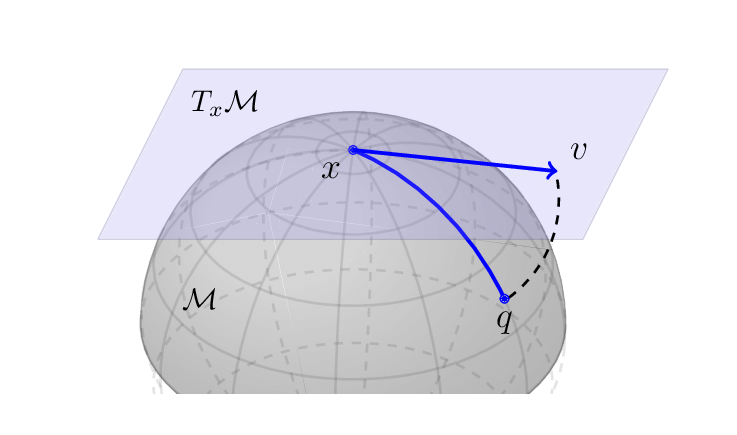
\includegraphics[width=\linewidth]{images/Figure-S3-Geometric-illustration-of-tangent-vector-tangent-space-curve-and.png}
    \caption{A hemispherical surface, $M$, with a tangent plane taken at point $z$. This tangent plane is in the tangent space of $M$.}
    \label{fig:tangent_space}
\end{marginfigure}

\subsection{Transformation of Basis Vectors}
Consider some arbitrary $\vec{A}$, with corresponding components and basis vectors
\begin{align*}
    \vec{A} & = A^\alpha \vec{e}_\alpha \\ & = A^{\alpha'} \vec{e}_{\alpha '} \\ & = \frac{\partial x^{\alpha'}}{\partial x^\alpha} A^\alpha \vec{e}_{\alpha'}
\end{align*}
Since $\vec{A}$ and $A^\alpha$ are equally arbitrary:
\begin{definition}[Transformation of Basis Vector]
    The transformation of a primed basis vector to unprimed basis vector is given by
    $$ \vec{e}_\alpha = \frac{\partial x^{\alpha'}}{\partial x^\alpha} \vec{e}_{\alpha'} $$
\end{definition}

\section{One-forms}
A 1-form, denoted by a letter with a tilde, e.g. $\widetilde{p}$, has three equivalent definitions, similar to vectors. These are:
\begin{itemize}
    \item A coordinate independent object with 4 linearly independent components, corresponding to the 4 coordinates in spacetime.
    \item A coordinate independent object, who's components transform like components of a gradient.
    \item A type $\binom{0}{1}$ tensor, which accepts vectors as arguments, and returns a real number.
\end{itemize}

Much like was mentioned earlier with vectors, a 1-form is a local object, since the contours that it represents must be straight. These contours must be evenly spaced and straight.
\subsection{One-form components}
A component of a 1-form is defined as 
$$ p_\alpha = \widetilde{p}(\vec{e}_\alpha) $$
Consider some arbitrary vector $\vec{A}$, and the relation between vectors and 1-forms can be shown as follows
\begin{align*}
    \widetilde{p}(\vec{A}) & = \widetilde{p}(A^\alpha \vec{e}_\alpha) \\ & = A^\alpha \widetilde{p}(\vec{e}_\alpha) && \text{(linearity)} \\ & = A^\alpha p_\alpha && \text{(definition)}
\end{align*}
There is a duality between vectors and 1-forms. They both exist in a tangent space for a point, and are dual to each other since a inner product may be taken between them. This inner product is the contraction
\begin{definition}[Inner Product]
    The contraction is an inner product, i.e.
    $$ \widetilde{p}(\vec{A}) = A^\alpha p_\alpha = \langle \widetilde{p}, \vec{A} \rangle $$
    Note that this is not the dot-product between vectors, since the dot-product requires a metric.
\end{definition}
$p_\alpha$ can be found then by creating a system of four simultaneous equations, and then solved to find each component.

\subsection{Transformation of 1-Forms Components}
Consider 1-form components of some primed index,
\begin{align*}
    p_{\alpha'} & = \widetilde{p}(\vec{e}_{\alpha'}) && \text{(definition)} \\
    & = \widetilde{p}\left(\frac{\partial x^\alpha}{\partial x^{\alpha'}} \vec{e}_\alpha \right) && \text{(change of vector basis)} \\ 
    & = \frac{\partial x^\alpha}{\partial x^{\alpha'}} \widetilde{p}  (\vec{e}_\alpha) && \text{(linearity)} \\ & = \frac{\partial x^\alpha}{\partial x^{\alpha'}} p_\alpha
\end{align*}
and thus it can be seen that 1-form components transform via the following identity
\begin{definition}[1-Form Component Transformation]
    The transformation of a 1-form components from a primed to unprimed space is given as
    $$ p_{\alpha} = \frac{\partial x^{\alpha'}}{\partial x^\alpha} p_{\alpha'} $$
\end{definition}

\subsection{Construction of $\widetilde{p}$ Components}
Similar to the vectors being constructed using basis vectors, the 1-forms are constructed using basis 1-forms.

\begin{definition}[Basis 1-Form]
    Basis 1-forms are written using the following notation
    $$ \gform{\omega}{\alpha} $$
    and are used to construct the 1-forms as follows
    $$ \widetilde{p} = p_\alpha  \gform{\omega}{\alpha} $$
\end{definition}

Similarly to basis vectors, the way to construct the basis 1-forms requires the formation of a family of linear equations, from which the values of the basis 1-forms can be found. 
\newpage
Now, consider an arbitrary vector $\vec{A}$ and 1-form $\widetilde{p}$:
\begin{align*}
        \widetilde{p}(\vec{A}) & = \widetilde{p}(A^\alpha \vec{e}_\alpha) && \text{(definition of vector} \\ 
        & = A^\alpha \widetilde{p}(\vec{e}_\alpha) &&\text{(linearity)} \\
        & = A^\alpha p_\beta \gform{\omega}{\beta} (\vec{e}_\alpha)
\end{align*}
Since $\vec{A}$ and $\widetilde{p}$ were taken to be arbitrary above,
$$ \gform{\omega}{\beta}(\vec{e}_\alpha) = \gvec{\delta}{\beta}{\alpha} $$
which forms a family of 16 linear equations which can be solved to find the 16 components of the 4 basis 1-forms.

\subsection{Transformation of Basis 1-Forms}
The basis 1-forms transform similarly to vector components
\begin{definition}[Transformation of Basis 1-Forms]
    $$ \gform{\omega}{\alpha'} = \frac{\partial x^{\alpha'}}{\partial x^\alpha} \gform{\omega}{\alpha} $$
\end{definition}

\subsection{1-Form Example}
The gradient 1-form is a common 1-form, somewhat analogous to the displacement vector. Consider some trajectory in spacetime, parameterised by an affine parameter, $\lambda$
$$ x^0(\lambda), \cdots, x^3(\lambda) $$
Similarly, consider an arbitrary scalar function, $\phi$, of the coordinates. The question is then of \textit{how does $\phi$ change along the trajectory?}
$$ \frac{d\phi}{d\lambda} = \frac{\partial \phi}{\partial x^\alpha} \frac{d x^\alpha}{d\lambda} $$
which is obvious via the chain rule. Looking at the individual components:
\begin{description}
    \item[$\frac{d\phi}{d\lambda}$] $\Rightarrow$ A pure number, coordinate independent
    \item[$\frac{d x^\alpha}{d\ \lambda}$] $\Rightarrow$ A vector component, as $dx$ is a known vector
    \item[$\frac{\partial \phi}{\partial x^\alpha}$] $\Rightarrow$ Via inspection, it is obvious this is a 1-form. It is the gradient 1-form.
\end{description}
\begin{corollary}[Gradient 1-Form]
    The gradient 1-form is written as
$$ \left(\widetilde{d\phi}\right)_\alpha $$
\end{corollary}

\subsection{Final Notes on 1-Forms}
\subsubsection{Gradient 1-form of basis vector}
If the scalar is chosen to be $\phi = x^\alpha$, an interesting identity will be arrived at, as follows:
\begin{align*}
    \langle \widetilde{d\phi}, \vec{e}_\beta \rangle & = \frac{\partial \phi}{\partial x^\gamma} \left(\vec{e}_\beta\right)^\gamma \\
    & = \frac{\partial x^\alpha}{\partial x^\gamma} \left(\vec{e}_\beta\right)^\gamma && \text{(from initial construction)} \\
    & = \gvec{\delta}{\alpha}{\gamma}\left(\vec{e}_\beta\right)^\gamma \\
    & = \gvec{\delta}{\alpha}{\gamma}\gvec{\delta}{\gamma}{\beta} \\
    & = \gvec{\delta}{\alpha}{\beta}
\end{align*}
and hence, $\widetilde{d\phi}$ with $\phi = x^\alpha$, is a basis 1-form.

\subsubsection{Normal Vector}
The normal vector is \textit{not} a fundamental property of a spacetime, since it needs a metric to `make sense'. Likewise, a gradient vector, like $\nabla$ for 3D, is  also not fundamental. \par However, a normal 1-form is fundamental, 
\begin{definition}[Normal 1-Form]
    The 1-form $\widetilde{n}$ is the normal 1-form if, $$\forall \vec{t} \in \text{tangent space}, \Tilde{n}(\vec{t}) = 0$$
\end{definition}

\section{General Tensors}
There are many ways to construct big tensors out of small tensors. For example:
\begin{itemize}
    \item Outer Product
    \item Derivatives
    \item (Anti) Symmetrise
\end{itemize}

Generally, a tensor of type $\binom{M}{N}$ is a multi-linear function of $M$ 1-forms and $N$ vectors, which returns a real number.

\subsection{Components of a Tensor}
They can be constructed by feeding in $M$ basis 1-forms, and $N$ basis vectors, for example a type $\binom{2}{3}$ tensor
$$ \gvec{T}{\alpha \beta}{\gamma \delta \epsilon} = T(\gform{\omega}{\alpha}, \gform{\omega}{\beta}, \vec{e}_\gamma, \vec{e}_\delta, \vec{e}_\epsilon) $$

\subsection{Outer Product}
The outer product of two vectors, noting that this can be generalised further, is defined as
$$ T = \vec{A} \otimes \vec{B} $$
which has the relation defined as
$$ T(\Tilde{p}, \Tilde{q}) \equiv \vec{A}(\Tilde{p}) \; \vec{B}(\Tilde{q}) $$
which, when evaluated, gives a real number.
\par The components of the outer product are defined as
$$ \gvec{T}{\alpha \beta}{} - A^\alpha B^\beta $$
Some important properties are as follows
\subsubsection{Symmetry}
The outer product \textbf{is not symmetric}, i.e. for the product 
$$ S = \vec{B} \otimes \vec{A} $$, then using the earlier definition,
$$ S(\Tilde{p}, \Tilde{q}) \neq T(\Tilde{p}, \Tilde{q}) $$

\subsubsection{Linear Combinations}
All type $\binom{2}{0}$ tensors may not be able to be written as an outer product, however, they can always be written as a linear combination of outer products, i.e. a type $\binom{M}{N}$ tensor can be written as a linear combination of $M$ vector outer products and $N$ 1-form outer products.

\subsubsection{Symmetrise}
An tensor can be symmetrised, or antisymmetrised. They are defined as follows
\begin{align*}
    T^{(sym)}(\Tilde{p}, \Tilde{q}) = T^{(\alpha \beta)} & = \frac{1}{2}\left[T(\Tilde{p}, \Tilde{q}) + T(\Tilde{p}, \Tilde{q})\right] \\
    T^{(anti)}(\Tilde{p}, \Tilde{q}) = T^{[\alpha \beta]} & = \frac{1}{2}\left[T(\Tilde{p}, \Tilde{q}) - T(\Tilde{p}, \Tilde{q})\right]
\end{align*}
\newpage
\section{Metric tensor and scalar product}
The metric is a tensor of type $\binom{0}{2}$, and described the dot product. As a consequence, it gives way to lengths and angles. It is defined as
\begin{definition}[Metric Tensor]
The metric tensor is a $\binom{0}{2}$ tensor:
    $$ g(\vec{A}, \vec{B}) \equiv \vec{A}\cdot\vec{B} $$
Who's components are described as 
$$ g_{\alpha \beta} = g(\vec{e}_\alpha, \vec{e}_\beta) = \vec{e}_\alpha \cdot \vec{e}_\beta $$
\end{definition}
Considering some infinitesimal displacement, the metric tensor then gives the spacetime interval, i.e.
\begin{align*}
    ds^2 & = g(d\vec{x}, d\vec{x}) \\ & = g_{\alpha \beta} dx^\alpha dx^\beta
\end{align*}
\subsubsection{Orthogonality}
Two vectors $\vec{A}$ and $\vec{B}$ are orthogonal if 
$$ g(\vec{A}, \vec{B}) = 0 $$
note that the orthogonal vectors need not be perpendicular, i.e. null vectors are orthogonal to themselves, but are not considered perpendicular.
\subsubsection{Null Vector}
A vector $\vec{A}$ is considered null if
$$ g(\vec{A}, \vec{A}) = 0 $$
An example of a null vector is the 4-momentum of a photon, where $\vec{p}\cdot \vec{p} = 0$.
\subsubsection{Basis Vector Lengths}
In general, $\vec{e}_\alpha$ doesn't have unit length, i.e.
$$ \vec{e}_\alpha \cdot \vec{e}_\alpha \neq 0 $$
and the basis vectors have different length, i.e. $\vec{e}_\alpha \cdot \vec{e}_\beta$ may vary. \par 
To measure the length of the basis vector components, one needs to inspect both the values and the metric.

\section{Covariant Derivative of Vector}
A local covariant derivative will be constructed in a flat tangent space to some point in spacetime. It turns out that this rule holds in curved spacetime, due to curvature being a 2nd order effect, vs the 1st order derivative. \par Consider some curve $x^0(\lambda), \dots, x^3(\lambda)$ in tangent space, which is parameterised by the affine parameter $\lambda$. \par Also consider a vector field, $\vec{V}$, which is defined with respect to the coordinates. \par The question is now of the change of $\vec{V}$ along the curve.
\begin{align*}
    \frac{d\vec{V}}{d\lambda} & = \frac{d}{d\lambda} (V^\alpha \vec{e}_\alpha) \\ 
    & = \frac{dV^\alpha}{d\lambda} \vec{e}_\alpha + V^\alpha \frac{d \vec{e}_\alpha}{d\lambda} \\
    & = \frac{\partial V^\alpha}{\partial x^\beta} \frac{d x^\beta (\lambda)}{d\lambda} \vec{e}_\alpha + V^\alpha \frac{\partial \vec{e}_\alpha}{\partial x^\beta} \frac{dx^\beta (\lambda)}{d\lambda}
\end{align*}
It is then important to note that
$$ \frac{\partial \vec{e}_\alpha}{\partial x^\beta} $$
is a vector. Hence, it can be written as a linear combination of the basis vectors
$$ \frac{\partial \vec{e}_\alpha}{\partial x^\beta} = \gvec{\Gamma}{\mu}{\alpha \beta} \vec{e}_\mu $$
where $\gvec{\Gamma}{\mu}{\alpha \beta}$ are the \textbf{Christoffel Symbols}.
\par The \textbf{covariant derivative} can then be written as 
$$ \gvec{V}{\alpha}{; \beta} = \frac{\partial V^\alpha}{\partial x^\beta} + \gvec{\Gamma}{\alpha}{\beta \gamma} V^\gamma $$
then leading to the total derivative being
$$ \frac{dV^\alpha}{d\lambda} = \gvec{V}{\alpha}{; \beta} \frac{dx^\beta(\lambda)}{d\lambda} $$

\begin{definition}[Covariant Derivative of Vector]
    For a vector $\vec{V}$ of type $\binom{1}{0}$, it's derivative is defined as
    \begin{align*}
        \left( \nabla V \right)^\alpha_{\beta} & \equiv V^\alpha_{;\beta} \\
        & = \frac{\partial V^\alpha}{\partial x^\beta} + \gvec{\Gamma}{\alpha}{\gamma \beta} C_\gamma
    \end{align*}
    and the derivative along some vector $\vec{A}$
    $$ \left( \nabla_{\vec{A}} V \right)^{\alpha} = A^\beta V^\alpha_{;\beta} $$
\end{definition}
\subsection{Notes on Covariant Derivative of Vector}
\subsubsection{Component Types}
Neither $\frac{\partial V^\alpha}{\partial x^\beta}$ or $\gvec{\Gamma}{\alpha}{\gamma \beta}$ are components of tensors, but $\gvec{V}{\alpha}{;\beta}$ is a tensor.
\subsubsection{Christoffel Symbols}
Christoffel symbols are defined by
$$ \frac{\partial \vec{e}_\alpha}{\partial x^\beta} = \gvec{\Gamma}{\mu}{\alpha \beta} \vec{e}_\mu $$
Then the components of $\Gamma$ are found by solving the 16 equations. There is another method of retrieving $\Gamma$ from $g$, which will be explored later.
\subsubsection{Physical Interpretation of the Covariant Derivative}
$\nabla \vec{A}$ is the rate of change, independent of coordinates. Furthermore $\gvec{\Gamma}{\alpha}{\beta \gamma} A^\gamma$ is the amount by which you need to `undo' $\frac{\partial A^\alpha}{\partial x^\beta}$ to obtain the coordinate independent change in $\vec{A}$.

\section{Covariant Derivative of 1-Form}
Again, consider some curve $x^0(\lambda), \dots, x^3(\lambda)$, and a 1-form $\Tilde{p}$. We will then ask to find it's change along the path.
$$
    \frac{d \Tilde{p}}{d\lambda} = \frac{\partial p_\alpha}{\partial x^\beta} \frac{d x^\beta (\lambda)}{d \lambda} \gform{\omega}{\alpha} + p_\alpha \frac{\partial \gform{\omega}{\alpha}}{\partial x^\beta} \frac{d x^\beta(\lambda)}{d\lambda} $$
Taking the 1-form of $\frac{\partial \gform{\omega}{\alpha}}{\partial x^\beta}$ and expanding it
$$ \frac{\partial \gform{\omega}{\alpha}}{\partial x^\beta} = \gvec{\chi}{\alpha}{\beta \mu} \gform{\omega}{\mu} $$
This new 1-form version of the Christoffel Symbols, $\gvec{\chi}{\alpha}{\beta \mu}$, can be related to the Christoffel Symbols using the orthogonality of bases.
$$ \gvec{\delta}{\alpha}{\beta} = \langle \gform{\omega}{\alpha}, \vec{e}_\beta \rangle $$
We then take the derivative with respect to some coordinate $x^\gamma$.
\begin{align*}
    0 & = \langle \frac{\gform{\omega}{\alpha}}{\partial x^\gamma}, \vec{e}_\beta \rangle + \langle \gform{\omega}{\alpha}, \frac{\vec{e}_\beta}{\partial x^\gamma} \rangle \\ & = \langle \gvec{\chi}{\alpha}{\gamma \mu} \gform{\omega}{\mu}, \vec{e}_\beta \rangle + \langle \gform{\omega}{\beta}, \gvec{\Gamma}{\nu}{\beta \gamma} \vec{e}_\nu\rangle \\ & = \gvec{\chi}{\alpha}{\gamma \mu} \langle\gform{\omega}{\mu}, \vec{e}_\beta \rangle + \gvec{\Gamma}{\nu}{\beta \gamma} \langle \gform{\omega}{\beta},  \vec{e}_\nu\rangle \\ & = \gvec{\chi}{\alpha}{\gamma \beta} + \gvec{\Gamma}{\alpha}{\beta \gamma}
\end{align*}
And thus $\chi$ and $\Gamma$ are opposite. It is important to note that they are symmetric in bottom indices. Finally, the definitions for covariant derivatives of 1-forms are found
\begin{definition}[Covariant Derivative of 1-Form]
    For a 1-form $\Tilde{p}$, it's derivative is defined as
    \begin{align*}
        \left( \nabla \Tilde{p} \right)_{\alpha \beta} & \equiv p_{\alpha \; ;\beta} \\
        & = \frac{\partial p_\alpha}{\partial x^\beta} - \gvec{\Gamma}{\gamma}{\alpha \beta} p_\gamma
    \end{align*}
    and the derivative along some vector $\vec{A}$
    $$ \left( \nabla_{\vec{A}} \Tilde{p} \right)_{\alpha} = A^\beta p_{\alpha\; ;\beta} $$
\end{definition}

\section{What is $\nabla g$?}
The goal is to find how the machine that measures lengths and angles, the metric $g$, changes as the spacetime changes. We can relate the covariant derivative of a vector and a 1-form using the metric as follows
$$ \nabla_{\vec{A}} \Tilde{V} = g(\nabla_{\vec{A}} \vec{V}, \dots) $$
with the following components
$$ A^\beta V_{\alpha \, ;\beta}  = g_{\alpha\gamma} \gvec{V}{\gamma}{;\beta}A^\beta $$
which gives an explanation, using geometric objects, for the `lowering' of indices, i.e. 
\begin{equation}
\label{eq:lowering}
    V_{\alpha \,;\beta} = g_{\alpha \gamma} \gvec{V}{\gamma}{;\beta}
\end{equation}
\par Now that the pre-work has been done, we are ready to calculate $\nabla g$.

\subsection{Calculating $\nabla g$}
We will begin with the standard identity
$$ V_\alpha = g_{\alpha \gamma} V^\gamma $$
Then, taking the covariant derivative with respect to $x^\beta$ on both sides, which gives
\begin{align*}
    V_{\alpha \,;\beta} & = g_{\alpha\gamma \,;\beta} V^\gamma + g_{\alpha \gamma} \gvec{V}{\gamma}{;\beta} \\ & = g_{\alpha\gamma \,;\beta} V^\gamma + V_{\alpha ; \beta} && \text{(from \vref{eq:lowering})} \\ 
    \Rightarrow g_{\alpha\gamma \,;\beta} & = 0
\end{align*}
\marginnote{The comma in the notation refers to a standard partial derivative with respect to $x^\gamma$ in this case.}
This shows that the tool for measuring lengths foes no change from one point in spacetime to another. However, the coordinate expression does change.
Written in terms of Christoffel Symbols
\begin{equation}
\label{eq:christoffel_g}
    0 = g_{\alpha \beta, \gamma} - \gvec{\Gamma}{\mu}{\alpha \gamma} g_{\mu \beta} - \gvec{\Gamma}{\nu}{\beta \gamma} g_{\alpha \nu}
\end{equation}

\subsection{Notes on $\nabla g$}
\subsubsection{Equivalence}
Since we know $g_{\alpha \beta, \gamma}$ in Minkowski, since $g_{\alpha \beta} = diag(-1, 1, 1, 1)$. It is also known that $\Gamma$ = 0 in Minkowski, since basis vectors are constant.  Hence, the right hand side of \vref{eq:christoffel_g} is zero in Minkowski. Furthermore, since this is expressed as a tensor equation of geometric objects, it must be true in all coordinates. \par This is the \textbf{Principle of Equivalence}.
\subsubsection{Christoffel Symbol Values}
In \vref{eq:christoffel_g}, the Christoffel symbols are made of 64 equations with 40 independent values, due to symmetry. This is true for the terms of $g$ and $\Gamma$. These equations can then be solved to find the terms of the Christoffel Symbols from the metric
$$ \gvec{\Gamma}{\mu}{\alpha \beta} = \frac{1}{2}g^{\mu \lambda} \left(g_{\lambda \alpha, \beta} + g_{\lambda \beta, \alpha} - g_{\alpha \beta, \lambda}\right) $$
where $g^{\mu \lambda}$ is the inverse metric.
\setchapterstyle{kao}
\setchapterpreamble[u]{\margintoc}
\chapter{Kinematics}
Kinematics refer to the motion of an object with respect to a given metric.
\begin{definition}[Displacement]
    The displacement is defined as
    $$ ds^2 = g(d\Vec{x}, d\Vec{x}) $$
\end{definition}
\section{Events and Intervals}
\begin{figure}[!ht]
\centering
\resizebox{0.6\textwidth}{!}{%
\begin{circuitikz}
\tikzstyle{every node}=[font=\large]

\draw [ color={rgb,255:red,122; green,122; blue,122}, , line width=1.2pt](12.5,15.75) to[short] (12.5,7);
\draw[ color={rgb,255:red,122; green,122; blue,122}, , line width=1.2pt] (20.75,9) to[short] (10.25,9);
\draw [line width=2pt, short] (19.5,14.75) -- (10.5,7.75);
\draw [line width=2pt, short] (19.5,8) -- (10.5,14.75);
\draw [line width=0.9pt, ->, >=Stealth] (18.75,11.25) -- (15.75,11.25)node[pos=0, fill=white]{Event P};
\draw [ color={rgb,255:red,170; green,121; blue,66} , fill={rgb,255:red,170; green,121; blue,66}, line width=1.5pt ] (14,14.25) circle (0.25cm);
\draw [ color={rgb,255:red,170; green,121; blue,66} , fill={rgb,255:red,170; green,121; blue,66}, line width=1.5pt ] (19.25,9.75) circle (0.25cm);
\draw [ color={rgb,255:red,170; green,121; blue,66} , fill={rgb,255:red,170; green,121; blue,66}, line width=1.5pt ] (17.25,13) circle (0.25cm);
\node [font=\large] at (14.75,14.75) {$Q_1$};
\node [font=\large] at (18,12.75) {$Q_3$};
\node [font=\large] at (18.5,9.75) {$Q_2$};
\end{circuitikz}
}%
\label{fig:causality}
\end{figure}
The above plot shows the possible types of relations between points and an event that can occur. These are
\begin{description}
    \item[$Q_1$] - \textbf{Timelike} relative to $P$, where $ds^2 < 0$, i.e. $Q_1$ can be reached from $P$. Equivalently, there exists a coordinate system where $Q_1$ and $P$ are at the same spatial location, but at different times.
    \item[$Q_2$] - \textbf{Spacelike} relative to $P$, where $ds^2 > 0$, i.e. $Q_2$ cannot be reached from $P$ in a spaceship. Equivalently, there exists a coordinate system where $P$ and $Q_2$ occur at the same time, but different spatial locations.
    \item[$Q_3$] - \textbf{Lightlike}, i.e. $Q_3$ will be reached from $P$ by photons. 
\end{description}

\subsection{Proper Time}
Proper time is defined as an affine parameter which leads to a particular normalisation of $d\vec{x}$, and hence $ds$.
\begin{definition}[Proper Time]
    Proper time is defined as
    $$ d\tau = \left(-ds^2\right)^{\frac{1}{2}} $$
    which can also be written as
    $$ -d\tau^2 = d\vec{x}\cdot d\vec{x} $$
\end{definition}

\section{4-Velocity and 4-Acceleration}
Consider a projectile with a path
$$ x^0(\lambda), \dots, x^3(\lambda) $$
here parameterised with the affine parameter $\lambda$. We will from now use the affine parameter of \textbf{proper time} to parameterise this path.
\subsection{4-Velocity}
\begin{definition}[4-Velocity]
    4-Velocity is defined along a path with respect to the proper time
    $$ \vec{u} = \frac{d \vec{x}(\tau)}{d\tau} $$
    where $d\vec{x}(\tau)$ is the infinitesimal displacement from $\tau$ to $\tau + d\tau$
    From the property of proper time, there is a normalisation condition of
    $$ -1 = \vec{u} \cdot \vec{u} $$
\end{definition}
It can more clearly be seen here how proper time is simply the parametrisation of the trajectory that allows for this normalisation condition to hold.
\subsection{Examples of 4-Velocity}

\subsubsection{MCRF: Momentarily Comoving Reference Frame}
This case is one where the coordinate system is momentarily comoving with the particle, i.e. the particle is momentarily at rest (spatially). This is local. \par
The coordinates of the object in the MCRF are parameterised with respect to proper time, i.e.
$$ t(\tau), \dots, z(\tau) $$
where, from the property of this system
\begin{align*}
    u^t & = \frac{dt(\tau)}{d\tau} \neq 0 \\
    u^x & = \frac{dx(\tau)}{d\tau} = 0
\end{align*}
and the same for $u^y$ and $u^z$. \par Hence 
$$ \vec{u} = (u^t, 0, 0, 0) $$
where by applying the normalisation condition, without assuming the metric, gives
$$ -1 = g_{tt} (u^t)^2 $$
\begin{description}
    \item[Minkowski] -- $g_{tt} = -1 \Rightarrow u^t = 1$
    \item[Schwarzchild] -- $g_{tt} = - \left( 1 - \frac{2M}{r}\right) \Rightarrow u^t = \left(\sqrt{1 - \frac{2M}{r}}\right)^{-1} $
\end{description}
The interpretation of $u^t$ is that tick separation in the coordinate system compared to the tick separation in proper time.

\subsubsection{Coordinate System in which Particle Moves Instantaneously with Speed $V$ in the $x$ Direction}
Similarly to before we will set up the velocity components
\begin{align*}
    u^t & = \frac{dt(\tau)}{d\tau} \neq 0 \\
    u^x & = \frac{dx(\tau)}{d\tau} = \frac{dx}{dt}\frac{dt}{d\tau} = Vu^t
\end{align*}
Using the normalisation condition
$$ -1 = (u^t)^2 \left(g_{tt} + 2g_{tx} V + g_{xx} V^2 \right) $$
Where solving for $u^t$ will give the clock tick ratios.
\begin{description}
    \item[Minkowski] -- $u^t = \left(\sqrt{1-V^2}\right)^{-1}$ 
    \item[Schwartzchild] -- $u^t = \left[1 - \frac{2M}{r} - \frac{V^2}{1- \frac{2M}{r}} \right]^{-1/2}$
\end{description}

\subsection{4-Acceleration}
Acceleration can not be taken to be the derivative of velocity with respect to $\tau$, since the curvature `pollutes' the second derivative. Hence, it is taken as the covariant derivative of $\vec{u}$, taken along the $\vec{u}$ itself. This then considers the change of the velocity in the tangent space.
\begin{definition}[4-Acceleration]
    The 4-Acceleration is defined as
    $$ \vec{a} = \nabla_{\vec{u}} \vec{u} $$
\end{definition}

Note that in free-fall, acceleration is $0$.

\subsection{Orthogonality of $\vec{u}$ and $\vec{a}$}
In 3D, this is not generally true. However, in 4 dimensions, this holds. \par Begin with the  normalisation property of 4-velocity
$$ -1 = \vec{u} \cdot \vec{u} $$
and then take the covariant derivative along $\vec{u}$, $\nabla_{\vec{u}}$, to both sides
\begin{align*}
    0 & = \left(\nabla_{\vec{u}} \vec{u}\right) \cdot \vec{u} + \vec{u} \cdot \left(\nabla_{\vec{u}} \vec{u}\right) \\ & = 2\vec{a} \cdot \vec{u}
\end{align*}
and hence the orthogonality of 4-velocity and 4-acceleration is arrived at.
\begin{definition}[Orthogonality of 4-Velocity and 4-Acceleration]
\label{def:4_orthog}
    The following property holds in 4-dimensional spacetime
    $$ \vec{a}\cdot \vec{u} = 0 $$
\end{definition}

\subsection{Worked Examples}
\subsubsection{Spaceship hovering at constant radius $r$ above a black hole of mass $M$}

This example will make use of spherical polar coordinates. Since the spaceship is spatially static, the only non-zero component of the 4-velocity is $u^t$
$$ u^t = \left(1 - \frac{2M}{r}\right)^{-\frac{1}{2}} $$
which is arrived at via the normalisation requirement and using the Schwartzchild metric. \par
Now consider the components of $\vec{a}$
\begin{align*}
    a^\alpha & = u^\beta \gvec{u}{\alpha}{;\beta} \\
    & = \frac{dx^\beta}{d\tau} \left(\frac{\partial u^\alpha}{\partial x^\beta} + \gvec{\Gamma}{\alpha}{\gamma \beta} u^\gamma \right) \\
    & = \frac{du^\alpha}{d\tau} + \gvec{\Gamma}{\alpha}{\gamma \beta} u^\gamma u^\beta
\end{align*}
where the jump from line 2 to 3 is done so using the chain rule. \par Since $r$ is constant, $$ \frac{du^t}{d\tau} = 0 $$
Hence, the only non-zero component of the acceleration is the radial component
\begin{align*}
    a^r & = 0 + \gvec{\Gamma}{r}{tt} \left(u^t\right)^2 \\ 
    & = \frac{M}{r^2} \left(1- \frac{2M}{r}\right) \cdot \left(1 - \frac{2M}{r} \right)^{-1} \\
    \Rightarrow a^r & = \frac{M}{r^2}
\end{align*}
The interesting part of this result is that, compared to the classical Newtonian result, the sign has an opposite positivity, since in this curved spacetime, a free-falling object has zero acceleration, this result shows the acceleration needed to stay out of the well of the black hole.

\subsubsection{Uniform Acceleration in Minkowski Spacetime}
In this example, a spaceship moves along the x-axis (of global Minkowski spacetime) with constant proper acceleration $g$. \par For constant proper acceleration, define a local coordinate system whose clocks are proper, i.e. moving with the ship, and measure infinitesimal displacement and 4-velocity here, and therefore $\vec{a}$. \par
Defined this local coordinate as a \textit{momentary comoving reference frame}, as seen earlier, with Minkowski spacetime. \par Since the spaceship is spatially static in this comoving coordinate system
$$ u^t = 1 \quad u^x = u^y = u^z = 0 $$
which gives
$$ \vec{a} = \left(\frac{du^t}{d\tau}, \frac{du^\lambda}{d\tau}, 0, 0\right) $$
due to the orthogonality of 4-velocity and 4-acceleration, \vref{def:4_orthog}, the first term is $0$. This leaves $a^x$, which is $g$, the proper acceleration. \par
Note that this is all local, i.e. instantaneous local acceleration and velocity. To then solve for global trajectories, invariant quantities are needed. These, in Minkowski, are
\begin{align*}
    -1 & = \vec{u} \cdot \vec{u} \\
    0 & = \vec{u} \cdot \vec{a} \\
    g^2 & = \vec{a} \cdot \vec{a}
\end{align*}
Then solving for these gives rise to \textbf{Hyperbolic Motion}.
\begin{corollary}[Hyperbolic Motion]
    Hyperbolic motion is uniform acceleration in Minkowski spacetime. The path, parameterised by proper time $\tau$ is defined as
    \begin{align*}
        t(\tau) & = g^{-1} \sinh(g\tau) \\
        x(\tau) & = g^{-1} \cosh(g\tau) \\
        y(\tau) & = z(\tau) = 0
    \end{align*}
\end{corollary}

From this derivation of hyperbolic motion, it is obvious to see that a photon launched from $x(0) < 0$ never catches the ship, i.e. the light cone from the origin forms a horizon from the spaceship. \par More generally, if $\vec{a}$ is known along the trajectory, then one can solve for the trajectory. 
\begin{align*}
    \vec{a} & = \nabla_{\vec{u}} \vec{u} \\
    a^\alpha & = \gvec{u}{\alpha}{; \beta} u^\beta \\
    & = \frac{d u^\alpha}{d\tau} + \gvec{\Gamma}{\alpha}{\beta \gamma} u^\beta u^\gamma
\end{align*}
This forms 4 ODEs for components of $\vec{u}$, given the (known) components of the acceleration and the (known) components of the $\Gamma$'s. Note, however, that generally the $\Gamma$'s depend on the coordinate position of the body, so there are 8 ODEs. The above four, and 
$$ \frac{d x^\alpha(\tau)}{d\tau} = u^\alpha(\tau) $$

\subsubsection{Special Case: Free Fall}
In free fall, 
$$ \vec{a} = 0 $$
Generally, we can do as before, but to make the solution easier, it is also possible to look for constants of the motion. \par Starting from 
\begin{align*}
    0 & = \nabla_{\vec{u}} \vec{u} \\
    0 & = \nabla_{\vec{u}} \Tilde{u}
\end{align*}
which are the acceleration in free-fall, and it's associated 1-form result. From here 
\begin{align*}
    0 &= u_{\alpha \, ; \beta} u^\beta \\
    & = \frac{d u_\alpha}{d\tau} - \gvec{\Gamma}{\gamma}{\alpha\beta} u_\gamma u^\beta \\
    \Rightarrow \frac{d u_\alpha}{d\tau} & = \frac{1}{2} g^{\gamma \lambda} \left(g_{\lambda \alpha, \beta} + g_{\lambda \beta, \alpha} - g_{\alpha \beta, \lambda}\right) u_\gamma u^\beta \\ & = \frac{1}{2} \left(g_{\lambda \alpha, \beta} + g_{\lambda \beta, \alpha} - g_{\alpha \beta, \lambda}\right) u^\lambda u^\beta \\ & = \frac{1}{2}g_{\lambda \beta, \alpha} u^\lambda u^\beta
\end{align*}
\marginnote{Note that when there are anti-symmetric tensors multiplied by tensors that are symmetric, i.e. the first and third $g$ terms, they vanish.}
Which gives the result that $u_\alpha = const.$ if the metric is independent of $x^\alpha$. \par 
Free-fall is a special case of a more general mechanism called \textbf{parallel transport}. \par
If $x^0(\tau), \dots, x^3(\tau)$ describes a curve, then we \textbf{parallel transport} any vector, or tensor, $\vec{V}$, along the curve by solving 
$$ 0 = \nabla_{\vec{u}} \vec{V} $$
for the components $V^\alpha(\tau)$.



\section{Physical Measurements}
For a physical measurement to be meaningful/useful, it must be coordinate independent. Since the components of a geometric object are not coordinate independent, they cannot be directly associated with a physical measurement. \par The aim, therefore, is to express physical observables as contractions of tensors with no free indices left, and therefore making these quantities coordinates independent. \par Furthermore, all physical measurements are local, and so we can express them in local Minkowski coordinate, and then write them as a coordinate independent result. This result would then hold in arbitrary coordinates. Once again, the principle of equivalence has shown itself.
\setchapterstyle{kao}
\setchapterpreamble[u]{\margintoc}
\chapter{Calculus in Curvilinear Coordinates in Flat Space}

\section{Christoffel Symbols}
\subsection{Christoffel Symbols from the Metric}
\section{Covariant Derivative}

\setchapterstyle{kao}
\setchapterpreamble[u]{\margintoc}
\chapter{Curved Space}

% \section{Manifolds, Local Flatness, and Local Lorentz Invariance}
% \section{Lengths, Volumes, Divergence, and Gauss' Law}

\section{Fermi-Walker Transport}
For a spaceship travelling along a trajectory $x^0(\tau), \dots, x^3(\tau)$, let 
\begin{align*}
    \vec{u}(\tau) & = \frac{d\vec{x}}{d\tau} && \text{4-Velocity} \\
    \vec{a}(\tau) & = \nabla_{\vec{u}} \vec{u} && \text{4-Acceleration}
\end{align*}
Then the Fermi-Walker transport defined how any geometric object evolves if we put it in a spaceship and drive off with it. i.e. It ensures the only rotation of the spatial basis vectors is due to the proper acceleration of the coordinate system. \par It is defined as the solution to the system of ODEs resulting from
$$ \nabla_{\vec{u}} \vec{V} = \vec{u}\vec{a} \cdot \vec{V} - \vec{a}\vec{u} \cdot \vec{V} $$
This is solved given a $\vec{u}$ and $\vec{a}$. \par The properties if this are
\begin{enumerate}
    \item $\vec{V} \cdot \vec{V}$ is conserved along the trajectory. Furthermore, orthogonality is conserved. If $\vec{V}$ and $\vec{W}$ are orthogonal initially, then
    $$ \nabla_{\vec{u}} (\vec{V} \cdot \vec{W}) = 0 $$
    \item $\vec{u}$ is automatically Fermi-Walker transported. This is useful since $\vec{u}$ is timelike and can form one component of our transported coordinate axes.
    \item If $\vec{W}$ is spacelike, i.e. orthogonal to $\vec{u}$ and $\vec{a}$, then $\vec{W}$ doesn't evolve (`rotate') along the trajectory. Note, that there is no spatial rotation of $\vec{W}$, but there is a temporal rotation, e.g. two consecutive Lorentz boosts = one boost + one rotation.
\end{enumerate}

\section{Introduction to Curvature}
Consider a point $P$ on a curved spacetime. We wish to take the local metric $g_{\alpha\beta}$ and transform it into primed coordinates such that $g_{\mu'\nu'}$ is as flat as possible. \par We know this transformation, and it takes the form
$$ g_{\mu'\nu'} = \frac{\partial x^\alpha}{\partial x^{\mu'}} \frac{\partial x^\beta}{\partial x^{\nu'}} g_{\alpha \beta} $$
To consider the individual components of the transformation for different orders, i.e. see where this 'flattening' breaks down, we will take the Taylor expansion of the transformation around the point $P$.
\subsubsection{$0$th Order}
The goal here is to achieve Minkowski space, since this is the known $0$th order flat spacetime.
$$ \eta_{\mu' \nu'} = \frac{\partial x^\alpha}{\partial x^{\mu'}} \frac{\partial x^\beta}{\partial x^{\nu'}} \left. g_{\alpha \beta} \right|_P$$
We will define $\gvec{\Lambda}{\alpha}{\mu'} = \frac{\partial x^\alpha}{\partial x^{\mu'}}$, such that the above equation is satisfied. Is this possible? Yes, since $\gvec{\Lambda}{\alpha}{\mu'}$ has 16 free independent numbers, and $\eta_{\mu' \nu'}$ has 10 independent constraints. The 6 free degrees of freedom represent the 3 Lorentz boosts, and 3 rotations.

\subsubsection{1st Order}
Since we have already constrained the 1st order derivatives from the 0th order, there are only the 2nd order derivatives left to consider. 
$$ \frac{\partial^2 x^\beta}{\partial x^{\nu'} \partial x^{\lambda'}} $$
contains 40 independent numbers, and 
$$ g_{\mu' \nu', \lambda'} $$
contains 40 independent constraints. Thus, we have been successful in the 1st order. The lack of free numbers represents the principle of equivalence, when combined with the 0th order.

\subsubsection{2nd Order}
Now consider the goal of
$$ g_{\mu' \nu', \lambda' \gamma'} = 0 $$
Again, we already constrained the 2nd order derivatives, so now are left to consider the 3rd order, i.e. 
$$ \frac{\partial^3 x^\beta}{\partial x^{\nu'} \partial x^{\lambda'} \partial x^{\gamma'}} $$
which has 80 independent components.
Considering the metric, there are 100 constraint equations, and as such there are 20 irreducible degrees of freedom. These 20 degrees represent the components of curvature in 4D.

\section{Curvature}
There are two types of curvature
\begin{description}
    \item[Extrinsic] -- relies on embedded space, e.g. looking `from the outside' at a beach ball or cylinder.
    \item[Intrinsic] -- Curvature measured by experiments occurring completely in curved spacetime, e.g. do locally parallel lines converge or diverge?
\end{description}

% \section{Parallel Transport, Geodesics, and Fermi-Walker Transport}
% \section{Riemann Curvature Tensor and its Symmetries}
% \section{Weyl Tensor}
% \section{Bianchi Identites}
% \section{Ricci Tensor and Scalar}
\setchapterstyle{kao}
\setchapterpreamble[u]{\margintoc}
\chapter{Einstein's Gravity}

\section{History of the Theory}
\section{Review of the Equivalence Principle}
\section{Local and Global Reference Frames}
\section{Stress-Energy Tensor}
\section{Einstein's Field Equations}
\section{Cosmological Constant}
\section{Einstein-Hilbert Action}
\section{Alternative Gravities}
\section{Conservation Laws}
\section{Landau-Lifshitz Stress-Energy Pseudotensor}
\section{Numerical Relativity}
\setchapterstyle{kao}
\setchapterpreamble[u]{\margintoc}
\chapter{Weak Fields}

\section{Corrections of the Minkowski Metric}

\section{Gauge Transformations}

\addpart{Part 2: Terrestrial and Astronomical Applications}
\setchapterstyle{kao}
\setchapterpreamble[u]{\margintoc}
\chapter{General Relativistic Phenomena: Revisited}

\section{Gravitational Lensing}
\subsection{Macolensing}
\subsection{Microlensing}

\section{Gravitational Redshift}
\section{Pound-Rebka Experiment}
\section{Shapiro Delay}
\section{Cassini Satellite}
\section{Binary Pulsars}

\section{Mercury's Preihelion Shift}
\section{Periastron Shifts in Binary Pulsars}
\section{Frame Dragging}
\section{Lense-Thirring Precession}
\section{Gravity Probe B}
\section{Spin Angular Momentum}
\section{Geodetic Precession of a Binary Pulsar}
\section{Nordtvedt Effect}
\section{Lunar Ranging}

\section{Global Positioning System}

\setchapterstyle{kao}
\setchapterpreamble[u]{\margintoc}
\chapter{Gravitational Radiation}

\section{Plane-wave Propogations}
\section{Dispersion Relation in Vacuo and Medio}
\section{Polarization}
\section{Energy-Momentum Flux}

\section{Detection Physics}
\subsection{Modern Detectors}

\section{Generation}
\subsection{Green Function and Tails}
\subsection{Radiation Fields}
\subsection{Mass and Current Quadrapoles}
\subsection{Virial Theorem}

\section{Astrophysics}
\subsection{Stochastic Background}
\subsection{Compact Binary Coalescence}
\subsection{Supernovae}
\setchapterstyle{kao}
\setchapterpreamble[u]{\margintoc}
\chapter{Relativistic Stars}

\section{Oppenheimer-Volkoff Equation}

\section{Equation of State}
\subsection{Interior Solutions}
\subsection{Exterior Solutions}

\section{Stellar Collapse}
\section{Chandrasekhar Mass}
\section{Gravitational Redshift}

\section{Stellar Pulsations}

\section{Accretion Disks}
\section{Iron Spectral Lines}
\section{Ray Tracing}
\section{Sgr A*}
\setchapterstyle{kao}
\setchapterpreamble[u]{\margintoc}
\chapter{Black Holes}

\section{Nature of Singularities and Horizons}
\section{Penrose Diagram}
\section{Kruskal-Szekeres Coordinates}
\section{Solutions/Metrics}
\subsection{Schwarzschild}
\subsection{Kerr}
\subsection{Ressiner-Nordtsrom}
\subsection{Kerr-Newman}

\section{Kepler Problem}
\section{Energy Extraction}
\section{Blandford-Znajek Mechanism}

\setchapterstyle{kao}
\setchapterpreamble[u]{\margintoc}
\chapter{Cosmology in the Form of a "tweet"}

\section{Homogeneity}
\section{Isotropy}
\section{Friedmann-Robertson-Walker Metric}
\section{Friedmann Equations}
\section{Cosmological Expansion and Redshift}

\section{Modern Observations}
\subsection{Cosmic Microwave Background}
\subsection{Large-Sacel Structure}
\subsection{Big Bang Nucleosynthesis}
\setchapterstyle{kao}
\setchapterpreamble[u]{\margintoc}
\chapter{Beyond Classical Gravity (Non-examinable)}

\section{Extra Dimensions}
\section{Kaluza-Klein Theory}
\section{Black Holes in more than Four Dimensions}
\section{Inflation}
\section{String Theory}
%----------------------------------------------------------------------------------------

\backmatter % Denotes the end of the main document content
\setchapterstyle{plain} % Output plain chapters from this point onwards

%----------------------------------------------------------------------------------------
%	BIBLIOGRAPHY
%----------------------------------------------------------------------------------------

% The bibliography needs to be compiled with biber using your LaTeX editor, or on the command line with 'biber main' from the template directory

\defbibnote{bibnote}{Here are the references in citation order.\par\bigskip} % Prepend this text to the bibliography
\printbibliography[heading=bibintoc, title=Bibliography, prenote=bibnote] % Add the bibliography heading to the ToC, set the title of the bibliography and output the bibliography note

%----------------------------------------------------------------------------------------
%	NOMENCLATURE
%----------------------------------------------------------------------------------------

% The nomenclature needs to be compiled on the command line with 'makeindex main.nlo -s nomencl.ist -o main.nls' from the template directory

\nomenclature{$c$}{Speed of light in a vacuum inertial frame}
\nomenclature{$h$}{Planck constant}

\renewcommand{\nomname}{Notation} % Rename the default 'Nomenclature'
\renewcommand{\nompreamble}{The next list describes several symbols that will be later used within the body of the document.} % Prepend this text to the nomenclature

\printnomenclature % Output the nomenclature

%----------------------------------------------------------------------------------------
%	GREEK ALPHABET
% 	Originally from https://gitlab.com/jim.hefferon/linear-algebra
%----------------------------------------------------------------------------------------

\vspace{1cm}

{\usekomafont{chapter}Greek Letters with Pronunciations} \\[2ex]
\begin{center}
	\newcommand{\pronounced}[1]{\hspace*{.2em}\small\textit{#1}}
	\begin{tabular}{l l @{\hspace*{3em}} l l}
		\toprule
		Character & Name & Character & Name \\ 
		\midrule
		$\alpha$ & alpha \pronounced{AL-fuh} & $\nu$ & nu \pronounced{NEW} \\
		$\beta$ & beta \pronounced{BAY-tuh} & $\xi$, $\Xi$ & xi \pronounced{KSIGH} \\ 
		$\gamma$, $\Gamma$ & gamma \pronounced{GAM-muh} & o & omicron \pronounced{OM-uh-CRON} \\
		$\delta$, $\Delta$ & delta \pronounced{DEL-tuh} & $\pi$, $\Pi$ & pi \pronounced{PIE} \\
		$\epsilon$ & epsilon \pronounced{EP-suh-lon} & $\rho$ & rho \pronounced{ROW} \\
		$\zeta$ & zeta \pronounced{ZAY-tuh} & $\sigma$, $\Sigma$ & sigma \pronounced{SIG-muh} \\
		$\eta$ & eta \pronounced{AY-tuh} & $\tau$ & tau \pronounced{TOW (as in cow)} \\
		$\theta$, $\Theta$ & theta \pronounced{THAY-tuh} & $\upsilon$, $\Upsilon$ & upsilon \pronounced{OOP-suh-LON} \\
		$\iota$ & iota \pronounced{eye-OH-tuh} & $\phi$, $\Phi$ & phi \pronounced{FEE, or FI (as in hi)} \\
		$\kappa$ & kappa \pronounced{KAP-uh} & $\chi$ & chi \pronounced{KI (as in hi)} \\
		$\lambda$, $\Lambda$ & lambda \pronounced{LAM-duh} & $\psi$, $\Psi$ & psi \pronounced{SIGH, or PSIGH} \\
		$\mu$ & mu \pronounced{MEW} & $\omega$, $\Omega$ & omega \pronounced{oh-MAY-guh} \\
		\bottomrule
	\end{tabular} \\[1.5ex]
	Capitals shown are the ones that differ from Roman capitals.
\end{center}

%----------------------------------------------------------------------------------------
%	GLOSSARY
%----------------------------------------------------------------------------------------

% The glossary needs to be compiled on the command line with 'makeglossaries main' from the template directory

\setglossarystyle{listgroup} % Set the style of the glossary (see https://en.wikibooks.org/wiki/LaTeX/Glossary for a reference)
\printglossary[title=Special Terms, toctitle=List of Terms] % Output the glossary, 'title' is the chapter heading for the glossary, toctitle is the table of contents heading

%----------------------------------------------------------------------------------------
%	INDEX
%----------------------------------------------------------------------------------------

% The index needs to be compiled on the command line with 'makeindex main' from the template directory

\printindex % Output the index

%----------------------------------------------------------------------------------------
%	BACK COVER
%----------------------------------------------------------------------------------------

% If you have a PDF/image file that you want to use as a back cover, uncomment the following lines

%\clearpage
%\thispagestyle{empty}
%\null%
%\clearpage
%\includepdf{cover-back.pdf}

%----------------------------------------------------------------------------------------

\end{document}
